% Options for packages loaded elsewhere
\PassOptionsToPackage{unicode}{hyperref}
\PassOptionsToPackage{hyphens}{url}
%
\documentclass[
  doc,12pt,floatsintext]{apa7}
\usepackage{amsmath,amssymb}
\usepackage{iftex}
\ifPDFTeX
  \usepackage[T1]{fontenc}
  \usepackage[utf8]{inputenc}
  \usepackage{textcomp} % provide euro and other symbols
\else % if luatex or xetex
  \usepackage{unicode-math} % this also loads fontspec
  \defaultfontfeatures{Scale=MatchLowercase}
  \defaultfontfeatures[\rmfamily]{Ligatures=TeX,Scale=1}
\fi
\usepackage{lmodern}
\ifPDFTeX\else
  % xetex/luatex font selection
  \setmainfont[]{Times New Roman}
\fi
% Use upquote if available, for straight quotes in verbatim environments
\IfFileExists{upquote.sty}{\usepackage{upquote}}{}
\IfFileExists{microtype.sty}{% use microtype if available
  \usepackage[]{microtype}
  \UseMicrotypeSet[protrusion]{basicmath} % disable protrusion for tt fonts
}{}
\makeatletter
\@ifundefined{KOMAClassName}{% if non-KOMA class
  \IfFileExists{parskip.sty}{%
    \usepackage{parskip}
  }{% else
    \setlength{\parindent}{0pt}
    \setlength{\parskip}{6pt plus 2pt minus 1pt}}
}{% if KOMA class
  \KOMAoptions{parskip=half}}
\makeatother
\usepackage{xcolor}
\usepackage{color}
\usepackage{fancyvrb}
\newcommand{\VerbBar}{|}
\newcommand{\VERB}{\Verb[commandchars=\\\{\}]}
\DefineVerbatimEnvironment{Highlighting}{Verbatim}{commandchars=\\\{\}}
% Add ',fontsize=\small' for more characters per line
\usepackage{framed}
\definecolor{shadecolor}{RGB}{248,248,248}
\newenvironment{Shaded}{\begin{snugshade}}{\end{snugshade}}
\newcommand{\AlertTok}[1]{\textcolor[rgb]{0.94,0.16,0.16}{#1}}
\newcommand{\AnnotationTok}[1]{\textcolor[rgb]{0.56,0.35,0.01}{\textbf{\textit{#1}}}}
\newcommand{\AttributeTok}[1]{\textcolor[rgb]{0.13,0.29,0.53}{#1}}
\newcommand{\BaseNTok}[1]{\textcolor[rgb]{0.00,0.00,0.81}{#1}}
\newcommand{\BuiltInTok}[1]{#1}
\newcommand{\CharTok}[1]{\textcolor[rgb]{0.31,0.60,0.02}{#1}}
\newcommand{\CommentTok}[1]{\textcolor[rgb]{0.56,0.35,0.01}{\textit{#1}}}
\newcommand{\CommentVarTok}[1]{\textcolor[rgb]{0.56,0.35,0.01}{\textbf{\textit{#1}}}}
\newcommand{\ConstantTok}[1]{\textcolor[rgb]{0.56,0.35,0.01}{#1}}
\newcommand{\ControlFlowTok}[1]{\textcolor[rgb]{0.13,0.29,0.53}{\textbf{#1}}}
\newcommand{\DataTypeTok}[1]{\textcolor[rgb]{0.13,0.29,0.53}{#1}}
\newcommand{\DecValTok}[1]{\textcolor[rgb]{0.00,0.00,0.81}{#1}}
\newcommand{\DocumentationTok}[1]{\textcolor[rgb]{0.56,0.35,0.01}{\textbf{\textit{#1}}}}
\newcommand{\ErrorTok}[1]{\textcolor[rgb]{0.64,0.00,0.00}{\textbf{#1}}}
\newcommand{\ExtensionTok}[1]{#1}
\newcommand{\FloatTok}[1]{\textcolor[rgb]{0.00,0.00,0.81}{#1}}
\newcommand{\FunctionTok}[1]{\textcolor[rgb]{0.13,0.29,0.53}{\textbf{#1}}}
\newcommand{\ImportTok}[1]{#1}
\newcommand{\InformationTok}[1]{\textcolor[rgb]{0.56,0.35,0.01}{\textbf{\textit{#1}}}}
\newcommand{\KeywordTok}[1]{\textcolor[rgb]{0.13,0.29,0.53}{\textbf{#1}}}
\newcommand{\NormalTok}[1]{#1}
\newcommand{\OperatorTok}[1]{\textcolor[rgb]{0.81,0.36,0.00}{\textbf{#1}}}
\newcommand{\OtherTok}[1]{\textcolor[rgb]{0.56,0.35,0.01}{#1}}
\newcommand{\PreprocessorTok}[1]{\textcolor[rgb]{0.56,0.35,0.01}{\textit{#1}}}
\newcommand{\RegionMarkerTok}[1]{#1}
\newcommand{\SpecialCharTok}[1]{\textcolor[rgb]{0.81,0.36,0.00}{\textbf{#1}}}
\newcommand{\SpecialStringTok}[1]{\textcolor[rgb]{0.31,0.60,0.02}{#1}}
\newcommand{\StringTok}[1]{\textcolor[rgb]{0.31,0.60,0.02}{#1}}
\newcommand{\VariableTok}[1]{\textcolor[rgb]{0.00,0.00,0.00}{#1}}
\newcommand{\VerbatimStringTok}[1]{\textcolor[rgb]{0.31,0.60,0.02}{#1}}
\newcommand{\WarningTok}[1]{\textcolor[rgb]{0.56,0.35,0.01}{\textbf{\textit{#1}}}}
\usepackage{graphicx}
\makeatletter
\def\maxwidth{\ifdim\Gin@nat@width>\linewidth\linewidth\else\Gin@nat@width\fi}
\def\maxheight{\ifdim\Gin@nat@height>\textheight\textheight\else\Gin@nat@height\fi}
\makeatother
% Scale images if necessary, so that they will not overflow the page
% margins by default, and it is still possible to overwrite the defaults
% using explicit options in \includegraphics[width, height, ...]{}
\setkeys{Gin}{width=\maxwidth,height=\maxheight,keepaspectratio}
% Set default figure placement to htbp
\makeatletter
\def\fps@figure{htbp}
\makeatother
\setlength{\emergencystretch}{3em} % prevent overfull lines
\providecommand{\tightlist}{%
  \setlength{\itemsep}{0pt}\setlength{\parskip}{0pt}}
\setcounter{secnumdepth}{5}
% Make \paragraph and \subparagraph free-standing
\ifx\paragraph\undefined\else
  \let\oldparagraph\paragraph
  \renewcommand{\paragraph}[1]{\oldparagraph{#1}\mbox{}}
\fi
\ifx\subparagraph\undefined\else
  \let\oldsubparagraph\subparagraph
  \renewcommand{\subparagraph}[1]{\oldsubparagraph{#1}\mbox{}}
\fi
% definitions for citeproc citations
\NewDocumentCommand\citeproctext{}{}
\NewDocumentCommand\citeproc{mm}{%
  \begingroup\def\citeproctext{#2}\cite{#1}\endgroup}
\makeatletter
 % allow citations to break across lines
 \let\@cite@ofmt\@firstofone
 % avoid brackets around text for \cite:
 \def\@biblabel#1{}
 \def\@cite#1#2{{#1\if@tempswa , #2\fi}}
\makeatother
\newlength{\cslhangindent}
\setlength{\cslhangindent}{1.5em}
\newlength{\csllabelwidth}
\setlength{\csllabelwidth}{3em}
\newenvironment{CSLReferences}[2] % #1 hanging-indent, #2 entry-spacing
 {\begin{list}{}{%
  \setlength{\itemindent}{0pt}
  \setlength{\leftmargin}{0pt}
  \setlength{\parsep}{0pt}
  % turn on hanging indent if param 1 is 1
  \ifodd #1
   \setlength{\leftmargin}{\cslhangindent}
   \setlength{\itemindent}{-1\cslhangindent}
  \fi
  % set entry spacing
  \setlength{\itemsep}{#2\baselineskip}}}
 {\end{list}}
\usepackage{calc}
\newcommand{\CSLBlock}[1]{\hfill\break\parbox[t]{\linewidth}{\strut\ignorespaces#1\strut}}
\newcommand{\CSLLeftMargin}[1]{\parbox[t]{\csllabelwidth}{\strut#1\strut}}
\newcommand{\CSLRightInline}[1]{\parbox[t]{\linewidth - \csllabelwidth}{\strut#1\strut}}
\newcommand{\CSLIndent}[1]{\hspace{\cslhangindent}#1}
\ifLuaTeX
\usepackage[bidi=basic]{babel}
\else
\usepackage[bidi=default]{babel}
\fi
\babelprovide[main,import]{english}
\ifPDFTeX
\else
\babelfont{rm}[]{Times New Roman}
\fi
% get rid of language-specific shorthands (see #6817):
\let\LanguageShortHands\languageshorthands
\def\languageshorthands#1{}
% Manuscript styling
\usepackage{upgreek}
\captionsetup{font=singlespacing,justification=justified}

% Table formatting
\usepackage{longtable}
\usepackage{lscape}
% \usepackage[counterclockwise]{rotating}   % Landscape page setup for large tables
\usepackage{multirow}		% Table styling
\usepackage{tabularx}		% Control Column width
\usepackage[flushleft]{threeparttable}	% Allows for three part tables with a specified notes section
\usepackage{threeparttablex}            % Lets threeparttable work with longtable

% Create new environments so endfloat can handle them
% \newenvironment{ltable}
%   {\begin{landscape}\centering\begin{threeparttable}}
%   {\end{threeparttable}\end{landscape}}
\newenvironment{lltable}{\begin{landscape}\centering\begin{ThreePartTable}}{\end{ThreePartTable}\end{landscape}}

% Enables adjusting longtable caption width to table width
% Solution found at http://golatex.de/longtable-mit-caption-so-breit-wie-die-tabelle-t15767.html
\makeatletter
\newcommand\LastLTentrywidth{1em}
\newlength\longtablewidth
\setlength{\longtablewidth}{1in}
\newcommand{\getlongtablewidth}{\begingroup \ifcsname LT@\roman{LT@tables}\endcsname \global\longtablewidth=0pt \renewcommand{\LT@entry}[2]{\global\advance\longtablewidth by ##2\relax\gdef\LastLTentrywidth{##2}}\@nameuse{LT@\roman{LT@tables}} \fi \endgroup}

% \setlength{\parindent}{0.5in}
% \setlength{\parskip}{0pt plus 0pt minus 0pt}

% Overwrite redefinition of paragraph and subparagraph by the default LaTeX template
% See https://github.com/crsh/papaja/issues/292
\makeatletter
\renewcommand{\paragraph}{\@startsection{paragraph}{4}{\parindent}%
  {0\baselineskip \@plus 0.2ex \@minus 0.2ex}%
  {-1em}%
  {\normalfont\normalsize\bfseries\itshape\typesectitle}}

\renewcommand{\subparagraph}[1]{\@startsection{subparagraph}{5}{1em}%
  {0\baselineskip \@plus 0.2ex \@minus 0.2ex}%
  {-\z@\relax}%
  {\normalfont\normalsize\itshape\hspace{\parindent}{#1}\textit{\addperi}}{\relax}}
\makeatother

\makeatletter
\usepackage{etoolbox}
\patchcmd{\maketitle}
  {\section{\normalfont\normalsize\abstractname}}
  {\section*{\normalfont\normalsize\abstractname}}
  {}{\typeout{Failed to patch abstract.}}
\patchcmd{\maketitle}
  {\section{\protect\normalfont{\@title}}}
  {\section*{\protect\normalfont{\@title}}}
  {}{\typeout{Failed to patch title.}}
\makeatother

\usepackage{xpatch}
\makeatletter
\xapptocmd\appendix
  {\xapptocmd\section
    {\addcontentsline{toc}{section}{\appendixname\ifoneappendix\else~\theappendix\fi\\: #1}}
    {}{\InnerPatchFailed}%
  }
{}{\PatchFailed}
\usepackage{csquotes}
\geometry{a4paper,margin=25mm}
\setcounter{tocdepth}{2}
\linespread{1.5}
\fancyheadoffset[R,L]{0pt}
\raggedbottom
\usepackage[all]{nowidow}
\usepackage[bottom]{footmisc}
\interfootnotelinepenalty=10000
\usepackage{setspace}
\AtBeginEnvironment{tabular}{\doublespacing}
\usepackage{makecell}
\renewcommand{\cellset}{\renewcommand{\arraystretch}{0.7}}
\usepackage{pdfpages}
\ifLuaTeX
  \usepackage{selnolig}  % disable illegal ligatures
\fi
\usepackage{bookmark}
\IfFileExists{xurl.sty}{\usepackage{xurl}}{} % add URL line breaks if available
\urlstyle{same}
\hypersetup{
  pdftitle={Bayesian Linear Mixed Models for EEG analysis},
  pdflang={en-EN},
  hidelinks,
  pdfcreator={LaTeX via pandoc}}

\title{Bayesian Linear Mixed Models for EEG analysis}
\author{\phantom{0}}
\date{}


\shorttitle{Bayesian LMMs for EEG analysis}

\affiliation{\phantom{0}}

\begin{document}
\maketitle

\vspace{-20mm}
\begin{center}
\begin{figure}[h]
\begin{center}

\includegraphics[width=!,totalheight=!,scale=0.2]{hu_logo}
\end{center}
\end{figure}
\vspace*{5mm}
{\setstretch{1.5}
\textbf{Lebenswissenschaftliche Fakultät}\\
Institut für Psychologie\\
\vspace*{10mm}
}
{\setstretch{1.5}
\textbf{Bachelorarbeit}\\
zum Erwerb des akademischen Grades \\
Bachelor of Science (B.Sc.)\\
im Fach Psychologie\\
\vspace*{10mm}
}
\end{center}
\begin{flushleft}
{\setstretch{1.5}
\begin{tabular}{ll}
Vorgelegt von:&\textbf{Clara Behnke}\\
&Matrikelnummer: 621544\\
&clara.behnke$@$student.hu-berlin.de\\
&geb. am 19.02.2000 in Berlin\\
Erstprüferin:&Prof. Dr. Rasha Abdel Rahman\\
Zweitprüfer:&Dr. Martin Maier\\
&\\
Berlin, den xx.xx.2024&\\
\end{tabular}
}
\end{flushleft}

\clearpage

\mbox{}\thispagestyle{empty}\clearpage

\newpage

\thispagestyle{empty}

\vspace*{55mm}

\begin{center}\textbf{Acknowledgments}\end{center}

\ldots..

\clearpage

\mbox{}\thispagestyle{empty}\clearpage

\thispagestyle{empty}

\vspace*{10mm}

\begin{flushleft}
{\setstretch{1.0}
\tableofcontents
}
\end{flushleft}

\newpage

\setcounter{page}{5}

\section*{Abstract}\label{abstract}
\addcontentsline{toc}{section}{Abstract}

\noindent In many disciplines Bayesian methods have become increasingly important in complementing frequentist approaches to data analysis. This tutorial attempts to provide a comprehensible and approachable introduction to the use of Bayesian Linear Mixed Models for the analysis of EEG data. The basic concepts will be explained alongside a worked-out example of an analysis in R. The main components of this approach are the implementation of single trial-based analyses of event-related potentials as Bayesian Linear Mixed Models using the R package brms. Important aspects like the elicitation of appropriate priors and the implementation of model comparison will be addressed and possible extensions of the model introduced. All this in the attempt to provide a starting point for frequentist researchers to expand to Bayesian methods.

\emph{Keywords:} Bayesian statistics, Linear Mixed Models, EEG

\newpage

\section{Introduction}\label{introduction}

In many disciplines Bayesian methods have become increasingly important in complementing frequentist approaches to data analysis (e.g. Depaoli et al., 2017; Lee, 2011). The Bayesian framework comes with numerous advantages, providing for example a formalization closer to our natural way of thinking. In the analysis of EEG data, however, Bayesian methods have not yet been able to gain a foothold. While there were many advances in analyzing event-related potentials, a shift to Bayesian methods has not been one of them so far.

Traditionally, the nested structure of EEG data, each participants does the experiment for many trials, was analyzed with repeated measures ANOVAs. In recent years, however, linear mixed models (LMMs) became more and more popular to replace the ANOVAs (e.g., Frömer et al., 2018; Tibon \& Levy, 2015; Volpert-Esmond et al., 2021). LMMs come with several advantages over repeated measures ANOVAs, they allow for combinations of categorical and continuous variables (Frömer et al., 2018), they are more robust against unequal numbers of observations (Tibon \& Levy, 2015) and don't need the data to follow a specific variance structure for the sphericity assumption (Bagiella et al., 2000). LMMs also directly take into account individual differences between the participants. All of these advantages as well as advances in statistical software made LMMs the new state of the art in the analysis of psychophysiological data.

The use of Bayesian linear mixed models (BLMMs) makes it possible to keep all the advantages from frequentist LMMs while at the same time including the benefits of Bayesian methods. BLMMs are a flexible way to analyze nested data that allow the researcher to incorporate prior knowledge and quantify the uncertainty of the estimation (Bürkner, 2018; Kruschke, 2021). The purpose of this tutorial is to provide an accessible introduction to Bayesian Linear Mixed Models in the context of EEG data analysis and address frequently raised concerns about Bayesian methods.

\section{Using Bayesian Linear Mixed Models to Analyze Single Trial EEG Data}\label{using-bayesian-linear-mixed-models-to-analyze-single-trial-eeg-data}

To introduce BLMMs we will look at a hands-on example of analyzing event related potentials (ERPs), more specifically the N170 component, a common ERP component reacting to face perception (Eimer, 2011). The analysis starts with presenting the frequentist LMM as a comparison followed by an introduction and implementation of the BLMM. Aftwerwards, we are describing how to find appropriate priors and check model sensitivity as well as suggesting a model extension. Finally, we are introducing several ways of Bayesian hypothesis testing and presenting relevant reporting practices. The Bayesian analyses closely follow the digital book by Nicenboim et al. (n.d.) that provides a more detailed introduction to Bayesian methods for cognitive sciences. All the analyses were conducted in R ((\textbf{Rcoreteam?})) and the entire code can be downloaded from \url{https://github.com/behnkec/bayesian_lmm/}.

\subsection{Data Sets and Preprocessing}\label{data-sets-and-preprocessing}

As an example data set the N170 ERP component, a part of the ERP CORE data from Kappenmann and colleagues -Kappenman et al. (2021), was used. Forty participants (25 female, 15 male) from the University of California completed a visual discrimination task while continuous EEG was recorded using a Biosemi ActiveTwo recording system with 30 electrodes referenced to the mastoid. The participants were presented with pictures of faces and cars as well as scrambled faces and cars and had to distinguish between scrambled and non-scrambled stimuli by pressing a button. This task enables an isolation of the face-specific N170 component. For further details on the experiment see Kappenman et al. (2021).

The preprocessing was done using the single trial EEG pipeline of the \href{https://abdelrahmanlab.com/}{Abdel Rahman Lab for Neurocognitive Psychology}, Humboldt-Universität zu Berlin, that is based on Frömer et al. (2018) (see \url{https://github.com/alexenge/hu-neuro-pipeline}). For the N170 from the ERP CORE data set the sampling rate of the data was reduced to 250 Hz and the data were re-referenced from the online referencing to the mastoid to an offline average reference. As a result, the average over all EEG electrodes at any time point is zero while relative differences between different scalp areas are preserved. The ocular correction was done using an ICA with the \texttt{FastICA} algorithm. The data are filtered with a bandpass of 0.1 to 40 Hz by default and segmented in to epochs from -0.5 s to 1.5 s around the stimulus. Importantly, for every epoch the average voltage of the entire time window is subtracted from all time points of the epoch at each channel. Epochs will be rejected if the peak-to-peak amplitude exceeds 200 \(\mu\)V. Finally, the pipeline computes one single trial value for the ERP component of interest (the N170 for this data set) that consists of the average ERP amplitude across the time window of interest and the channels of the region of interest. This single trial average will be used as the dependent variable in the analyses. For the N170 the P08 was selected as the region of interest with a time window of 110 to 150 ms after stimulus onset as suggested in Kappenman et al. (2021). Additional information on the pipeline can be found in the documentation (see \url{https://hu-neuro-pipeline.readthedocs.io/en/latest/}). The code used for preprocessing can be found on GitHub.

In addition to the N170 component, the analyses were also performed for the N2 component using the data from Frömer et al. (2018). Adding another data set gives one the opportunity to review the procedure and check for subjectiveness. For ease of reading however the second data set will not be discussed further. The complete analysis for the N2 is accessible in the GitHub repository.

\subsection{Frequentist Linear Mixed Models}\label{frequentist-linear-mixed-models}

To provide a reference, we will start by performing the analysis with a frequentist linear mixed model. LMMs, also called multilevel models or mixed-effects models, are extensions of the general linear model (GLM) that additionally estimate random effects. They are used in situations, where the data have a nested or hierarchical structure and would violate the assumption of independent error terms in a standard linear regression. This is often the case in cognitive psychology when participants are presented with multiple stimuli. The same participant will do the experiment for several trials and these trials will therefore be more similar to each other than trials between participants. Each trial will not only be influenced by the experimental condition but also by individual differences between participants. The LMMs account for these individual differences by additionally estimating random effects. In contrast to fixed effects that are estimated in the GLM as well as in LMMs and generalize over the population, random effects estimate how much the intercept and/or slope of the regression varies between participants. If e.g.~the intercept is allowed to be random, that means that the intercept of every participant consists not only of the overall intercept but also an individual deviation of it.

In a basic form, LMMs include random effects only for the participants. However one could also add random effects for the items (or channels) as so called crossed random effects as described in Baayen et al. (2008). For reasons of simplicity and because item effects of pictures are usually small compared to the fixed effects and participant effects, in the present tutorial only random effects for participants will be included. However, it is important to note that setting up a sensible model and determining what random effects to include is a separate substantial issue and ongoing debate (see Barr et al., 2013; Bates et al., 2018; Matuschek et al., 2017).

\subsubsection{Mathematical Model and Implementation in R}\label{mathematical-model-and-implementation-in-r}

To set up the model, we need to formulate the hypothesis we are interested in and include the variables accordingly. In our example, we want to test the differences in the mean amplitude of the N170 after seeing a face or a car. Therefore, the mean amplitude of the N170 is our dependent variable and the experimental condition (seeing a picture of a face or of a car) is our predictor. Again, for reasons of simplicity, we will not include any other predictor, although this would of course be possible. As it is usually done, we allow for a correlation between random intercept and random slope.

In our simple case with only one predictor and random effects only for the participants, a linear mixed model can be described as in Eq. \eqref{eq:LMM}. The mean amplitude of the N170 \(Y_{ij}\) from trial \(i\) of participant \(j\) is predicted by a random intercept \(\beta_{0j}\) and the experimental condition \(X_{ij}\) that also has a random slope.

\begin{equation} 
Y_{ij} = \beta_{0j} + X_{ij} \cdot \beta_{1j} + \epsilon_{ij}
\label{eq:LMM}
\end{equation}

\begin{equation} 
\begin{split}
With \enspace & \beta_{0j} = \beta_{0} + u_{0j} \\
& \beta_{0j} = \beta_{0} + u_{0j} \\
& \beta_{1j} = \beta_{1} + u_{1j} \\
& u_0 \sim N(0, \tau_{u_0}) \\
& u_1 \sim N(0, \tau_{u_1}) \\
& cor(u_0, u_1) = \rho_u \\
& \epsilon \sim N(0, \sigma)
\end{split}
\label{eq:LMM-specifics}
\end{equation}

Eq. \eqref{eq:LMM-specifics} describes the random effects structure of the model. The random intercept consists of an fixed intercept \(\beta_{0}\) that is the same as for the standard linear regression as well as a person specific deviation \(u_{0j}\). This represents the variance of the intercept between participants and is normally distributed around zero with a standard deviation (sd) \(\tau_{u_0}\). The same concept applies to the effect of the predictor X which consists of a fixed effect \(\beta_{1}\) and a random effect \(u_{1j}\) that is also normally distributed around zero with an sd \(\tau_{u_1}\). Lastly, the correlation between random intercept and random slope is described by some \(\rho_u\). This correlation could also be assumed zero, but it is usually included in ERP research, so we will allow the random effects to correlate.

To fit the frequentist LMM in R, we will use the lmerTest package (Kuznetsova et al., 2017). We input our model into the \texttt{lmer} function by using the Wilkinson notation (Wilkinson \& Rogers, 1973) and specify the dataset.

\begin{Shaded}
\begin{Highlighting}[]
\CommentTok{\# Fitting the frequentist LMM}
\NormalTok{mod\_freq }\OtherTok{\textless{}{-}}\NormalTok{ lmerTest}\SpecialCharTok{::}\FunctionTok{lmer}\NormalTok{(N170 }\SpecialCharTok{\textasciitilde{}} \DecValTok{1} \SpecialCharTok{+}\NormalTok{ f\_c }\SpecialCharTok{+}\NormalTok{ (}\DecValTok{1} \SpecialCharTok{+}\NormalTok{ f\_c }\SpecialCharTok{|}\NormalTok{ participant\_id), }
                           \AttributeTok{data =}\NormalTok{ trials\_cond)}
\end{Highlighting}
\end{Shaded}

\subsubsection{Results}\label{results}

For easier comparison with the Bayesian models, we will look at the fixed and random effects of the frequentist model. A summary of all the model estimates can be found in Table \ref{tab:fLMM-table}. We defined the main fixed effect as the overall effect of the experimental condition. When participants were presented with faces the amplitude of the N170 component was significantly more negative, \(b_1 =\) -1.76, p \textless{} 0.001, compared to when presented with cars. For the random effects we are most interested in the standard deviations, as we will use those when setting up the Bayesian model. The sd of the random intercept was \(sd_0 =\) \texttt{4.129} and the sd of the random slope was \(sd_1 =\) \texttt{1.529} with a correlation of \(r =\) \texttt{0.07}. After fitting the Bayesian model we will be able to look at differences between the results of the two models.

\begin{table}[tbp]

\begin{center}
\begin{threeparttable}

\caption{\label{tab:fLMM-table}Results of Frequentist Linear Mixed Model}

\begin{tabular}{llllll}
\toprule
Term & \multicolumn{1}{c}{$\hat{\beta}$} & \multicolumn{1}{c}{95\% CI} & \multicolumn{1}{c}{$t$} & \multicolumn{1}{c}{$\mathit{df}$} & \multicolumn{1}{c}{$p$}\\
\midrule
Intercept & 5.69 & {}[4.39, 7.00] & 8.56 & 39.05 & < .001\\
F cface & -1.76 & {}[-2.35, -1.17] & -5.84 & 38.80 & < .001\\
\bottomrule
\end{tabular}

\end{threeparttable}
\end{center}

\end{table}

\subsection{Bayesian Linear Mixed Models}\label{bayesian-linear-mixed-models}

Bayesian Linear Mixed Models account for the same hierarchical structure as the frequentist LMMs seen above while at the same time incorporating the Bayesian framework. The basic idea of Bayesian statistics is to replace the point estimates we use in frequentist models with probability distributions. This allows us to incorporate prior knowledge into our estimation and update this knowledge using the collected data (van de Schoot et al., 2021). At the same time, Bayesian statistics allow us to directly model the uncertainty in our estimation.

\subsubsection{Mathematical Model}\label{mathematical-model}

The theorem known as Bayes' rule forms the basis of Bayesian statistics. The rule defines the calculation of a conditional probability \(p(A|B)\) of two events \(A\) and \(B\) given the probabilities of both individual events as well as the conditional probability \(p(B|A)\) (see Eq. \eqref{eq:bayes-rule}).

\begin{equation}
p(A|B) = \frac{p(B|A)p(A)}{p(B)}
\label{eq:bayes-rule}
\end{equation}

Bayes' rule can be extended by introducing vectors of parameters instead of single events into the equation. This extension now describes probability distributions rather than single probabilities. For a data set \(y\) and a set of model parameters \(\theta\) the extended Bayes' rule can be written as follows:

\begin{equation}
p(\theta|y) = \frac{p(y|\theta)p(\theta)}{p(y)}
\label{eq:bayes-rule-distributions}
\end{equation}

In Eq.\eqref{eq:bayes-rule-distributions}, the term \(p(\theta|y)\) stands for the posterior distribution (or simply posterior) and represents the conditional probability of the parameters given the data. This is the primary result of a Bayesian analysis and contains the entire information about possible parameter values. The posterior represents our updated belief after seeing the data. \(p(y|\theta)\) is called the likelihood and describes the data \(y\) as a function of the parameters \(\theta\). For every possible value the parameters can theoretically take, \(p(y|\theta)\) says how likely the data is, given this specific parameter value. The peak of this distribution, the maximum likelihood, is often used as an estimate in frequentist statistics. To compute the likelihood, we need to specify the underlying type of distribution of the data. Imagine modeling a coin toss. Usually one would think about the model in terms of the number of successes, e.g.~heads. We would use a binomial distribution to describe the probability of getting \(k\) heads given a certain probability of success \(\theta\). \(k\) would be the varying parameter in this perspective. The likelihood turns things around and assumes \(k\) to be fixed because the data was already collected and is therefore known. The varying parameter is now the probability of success \(\theta\) and likelihood represents the probability of getting the observed data given a certain \(\theta\). To model this we need to know the underlying distribution of the data. The term \(p(\theta)\) introduces the prior into the equation. The prior represents our knowledge about the parameters in the population before seeing any data. Specifying the prior is one of the primary challenges in Bayesian data analysis. Lastly, \(p(y)\) is called the marginal likelihood and can be thought of as an integral over the likelihood. The marginal likelihood works as a normalizing constant that ensures that the area under the curve of the posterior is equal to one, a prerequisite for the posterior to be a probability distribution.

After specifying a prior and deciding on a likelihood distribution, we can now compute the posterior distribution from the other three. In some cases, so called conjugate cases, the posterior can directly be derived analytically. Mostly though, this is not possible because the marginal likelihood is a complex integral, that cannot be computed analytically. That is why we will use statistical software to sample from the posterior distribution instead (see Section 2.6 for more details on sampling).

For the model specification we will drop the marginal likelihood, as it does not depend on the parameters \(\theta\) (van de Schoot et al., 2021). We can therefore describe the posterior as a distribution proportional to the likelihood multiplied by the prior (Eq. \eqref{eq:bayes-rule-proportional})

\begin{equation}
p(\theta|y) \sim p(y|\theta)p(\theta)
\label{eq:bayes-rule-proportional}
\end{equation}

We will now apply these concepts to LMMs. The basic model structure of dependent and independent variables as well as random effects remains the same, but we need to include the intracacies of Bayesian models. For the likelihood we will assume a normal distribution, as this approximately holds for single trial EEG averages (\textbf{Referenz???}). This is one other advantage of Bayesian models. If we wanted to model reaction times (which are usually not normally distributed), we could easily accommodate for any other distribution via the likelihood. Additionally, as for the frequentist LMM, we assume a linear relationship between the experimental condition and the EEG signal as well as some between-subject variability for the intercept and slope (Nicenboim et al., n.d.). For ease of writing we will directly include the random effects for intercept (\(u_{0j}\)) and slope (\(u_{1j}\)) into the equation. Equation \eqref{eq:BLMM} describes our model. Each observation \(Y_{ij}\) follows a normal distribution with a person specific mean. The mean is similar to the point estimate in the frequentist model, intercept and slope are both adjusted individually. The standard deviation \(\sigma\) of the normal distribution remains the same for every participant.

\begin{equation}
Y_{ij} \sim N(\beta_{0} + u_{0j} + X_{ij} \cdot (\beta_{1} + u_{1j}), \sigma)
\label{eq:BLMM}
\end{equation}

Based on this last equation (Eq. \eqref{eq:BLMM}) we need to set the following priors:

\begin{equation}
\begin{split}
& \beta_{0} \sim N(...,...) \\
& \beta_{1} \sim N(...,...) \\
& u_0 \sim N(0,\tau_{u_0}) \\
& u_1 \sim N(0,\tau_{u_1}) \\
& \tau_{u_0} \sim N_+(...,...) \\
& \tau_{u_1} \sim N_+(...,...) \\
& \rho_u \sim LKJcorr(...) \\
& \sigma \sim N_+(...,...)
\end{split}
\label{eq:priors-BLMM}
\end{equation}

For every parameter in our model our prior knowledge will be expressed as a prior and incorporated into the model. For the variance component of the random effects as well as of the overall distribution, we will use a truncated normal distribution because the standard deviation cannot take negative values. For the correlation we use a LKJ correlation distribution that is used to define correlation matrices (Joe, 2006; Lewandowski et al., 2009). This distribution takes only one parameter and smaller values result in a wider distribution. In section 2.4 we will discuss how to set appropriate priors for every parameter in more detail.

\subsubsection{Implementation in R}\label{implementation-in-r}

When fitting the Bayesian LMM in R the syntax stays almost the same as for frequentist LMMs. In the following example we are using the \texttt{brm} function from the brms package Bürkner (2024) to fit our model. This package relies on the statistical software STAN (Team, 2024) for the back-end computations. The sampling algorithm used by STAN is called Markov Chain Monte Carlo (MCMC) and will be discussed in more detail in Section 2.6. To use the \texttt{brm} function, we simply need to specify the prior and and set the likelihood distribution (\texttt{family}). In our case, we assumed single trial ERP averages to be normally distributed and we will therefore set the \texttt{family} to \texttt{gaussian}. This is also the default distribution, so technically we wouldn't have to specify it at all. Next, we need to specify a prior for every parameter of our model (see Eq. \eqref{eq:priors-BLMM}). At this moment we will assume the prior as given but the used prior will be derived in detail in the next section. The sampling will be done four independent times (so called chains) by default, with 2000 samples per chain. For each chain 1000 samples are discarded as a warm-up phase, which leads to a total of 4000 samples. To accelerate the computations we will set the \texttt{cores} argument to four, this parallelizes the computation by using one CPU for each chain (only if 4 CPUs are available).

\begin{Shaded}
\begin{Highlighting}[]
\CommentTok{\# Fitting the BLMM}
\NormalTok{mod\_blmm }\OtherTok{\textless{}{-}} \FunctionTok{brm}\NormalTok{(N170 }\SpecialCharTok{\textasciitilde{}} \DecValTok{1} \SpecialCharTok{+}\NormalTok{ f\_c }\SpecialCharTok{+}\NormalTok{ (}\DecValTok{1} \SpecialCharTok{+}\NormalTok{ f\_c }\SpecialCharTok{|}\NormalTok{ participant\_id), }\CommentTok{\# formula}
                \AttributeTok{data =}\NormalTok{ trials\_cond, }\CommentTok{\# data set}
                \AttributeTok{prior =}\NormalTok{ prior\_1, }\CommentTok{\# prior}
                \AttributeTok{family =} \FunctionTok{gaussian}\NormalTok{(), }\CommentTok{\# assumed likelihood distribution}
                \AttributeTok{cores =} \DecValTok{4}\NormalTok{) }\CommentTok{\# parallelization}
\end{Highlighting}
\end{Shaded}

\subsubsection{Results}\label{results-1}

To evaluate our model we will first take a look at the output of the \texttt{summary} function. This gives us an overview of all the important posterior distributions and convergence diagnostics.




\begin{verbatim}
##  Family: gaussian 
##   Links: mu = identity; sigma = identity 
## Formula: N170 ~ 1 + f_c + (1 + f_c | participant_id) 
##    Data: trials_cond (Number of observations: 6224) 
##   Draws: 4 chains, each with iter = 2000; warmup = 1000; thin = 1;
##          total post-warmup draws = 4000
## 
## Multilevel Hyperparameters:
## ~participant_id (Number of levels: 40) 
##                        Estimate Est.Error l-95% CI u-95% CI Rhat Bulk_ESS
## sd(Intercept)              4.33      0.52     3.44     5.48 1.00      964
## sd(f_cface)                1.59      0.29     1.09     2.20 1.00     2226
## cor(Intercept,f_cface)     0.07      0.19    -0.30     0.44 1.00     3105
##                        Tail_ESS
## sd(Intercept)              1526
## sd(f_cface)                2751
## cor(Intercept,f_cface)     2815
## 
## Regression Coefficients:
##           Estimate Est.Error l-95% CI u-95% CI Rhat Bulk_ESS Tail_ESS
## Intercept     5.67      0.71     4.25     7.06 1.01      568     1061
## f_cface      -1.76      0.31    -2.38    -1.13 1.00     2803     2664
## 
## Further Distributional Parameters:
##       Estimate Est.Error l-95% CI u-95% CI Rhat Bulk_ESS Tail_ESS
## sigma     7.06      0.06     6.94     7.19 1.00     6551     2980
## 
## Draws were sampled using sampling(NUTS). For each parameter, Bulk_ESS
## and Tail_ESS are effective sample size measures, and Rhat is the potential
## scale reduction factor on split chains (at convergence, Rhat = 1).
\end{verbatim}

\normalsize

The output is structured similarly to the output of a frequentist model. At the top, we can see the information we put into the model: the likelihood, the formula, the data and the sampling specifics. We did not specify a link function, so the identity function was used per default. The link function would allow to extend the model from a linear relationship to other relationships (extending it to a Generalized Linear Model (e.g. Nelder \& Wedderburn, 1972)), but we will not look at this kind of model.

Next, the output gives us the estimated posterior distributions of the random effects and the correlation between them. In Bayesian analyses, typically the entire distribution is used for inference. For a comparison with the frequentist model however, we can also look at the point estimates. For the random effects the point estimates of the standard deviation are very similar to what we have seen before. The sd of the random intercept was \(sd_0 =\) 4.33 (compared to \(sd_0 =\) \texttt{4.129}) and the sd of the random slope was \(sd_1 =\) 1.59 (compared to \(sd_1 =\) \texttt{1.529}) with a correlation of \(r =\) 0.07 (compared to \(r =\) \texttt{0.07}). We will ignore the rear columns of all the estimates for now. They contain convergence diagnostics and we will describe how to interpret them in section 2.6. Below the random effects are the fixed effects. Again, we can compare the point estimates to the frequentist model and notice a great similarity. When participants were presented with faces the amplitude of the N170 component was more negative, \(b_1\) = -1.76 (compared to \(b_1 =\) -1.76). What is new in the Bayesian summary is an estimate of sigma, the sd of the posterior normal distribution of the N170, at the end of the output. Here, the estimated sigma was \(\sigma =\) 7.06.

Finally, we can visualize the posterior distributions of the parameters of interest using the \texttt{plot} function (see Fig. \ref{fig:plot-blmm}). This allows for an overview of the entire posterior distribution and should always be part of a Bayesian analysis. The posterior distributions of our parameters give us information not only about the mean (or point estimate) of the distribution, but also the scale and shape as well as the range of the distribution. These help to better assess the model in its entirety. The \texttt{plot} function also outputs so called trace plots. The trace plots are a first indicator of the goodness of convergence (i.e.~if the algorithm used to compute the posterior distribution worked correctly). They should ideally be a straight hose around the mean of the estimation and should not have outliers.



\begin{Shaded}
\begin{Highlighting}[]
\FunctionTok{plot}\NormalTok{(mod\_blmm, }\AttributeTok{nvariables =} \DecValTok{6}\NormalTok{, }\AttributeTok{ask =} \ConstantTok{FALSE}\NormalTok{)}
\end{Highlighting}
\end{Shaded}

\begin{figure}
\centering
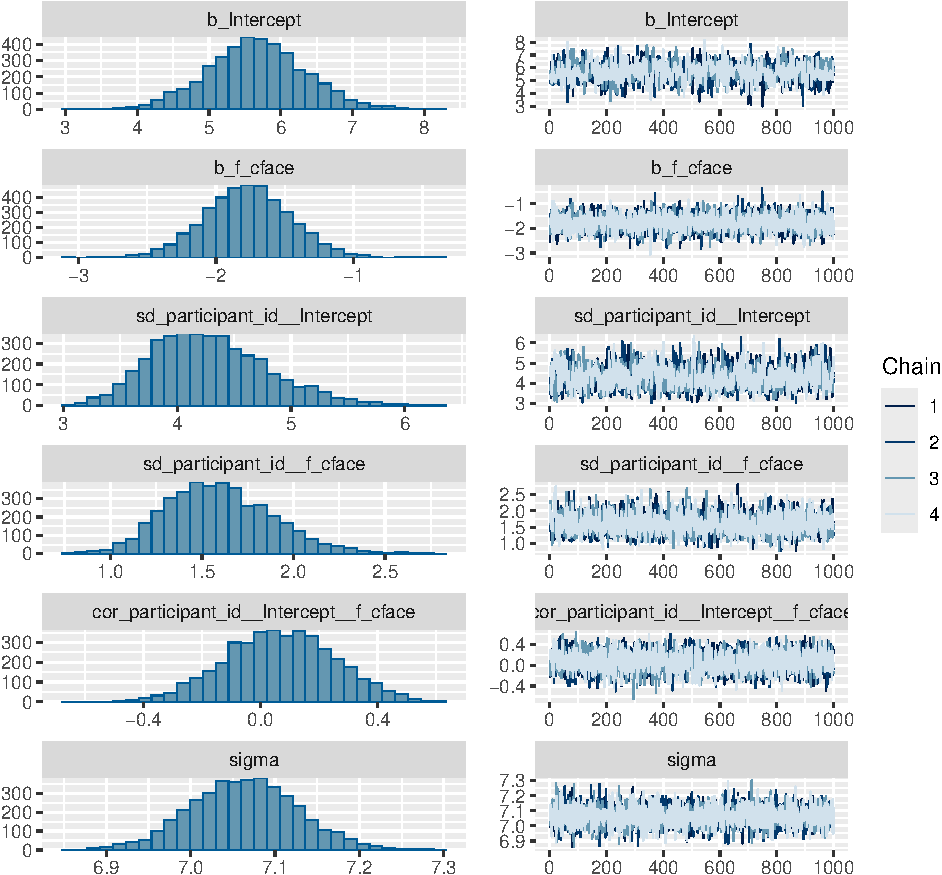
\includegraphics{bachelor_thesis_files/figure-latex/plot-blmm-1.pdf}
\caption{\label{fig:plot-blmm}Posterior distributions and trace plots of the correlation model}
\end{figure}

\subsection{Prior Elicitation}\label{prior-elicitation}

Probably the most frequently asked question about Bayesian statistics is how to determine the priors. For researchers with a frequentist background this often seems like a daunting task with a lot of subjectivity. However, while it does increase the researchers degrees of freedom and remains a difficult task even for expert statisticians, there are some paths you can follow to find appropriate priors. As we have seen in Section 2.3, prior distributions encode the knowledge about the parameters before seeing the data. Ideally prior distributions should therefore be elicited with no knowledge of the collected data incorporating only the available information before the measurement (Gelman et al., 2017). In the prior elicitation we are trying to translate this already available domain knowledge into probability distributions (Mikkola et al., 2023). In this process There are different approaches priors we choose can have different characteristics, depending on the approach In the following analysis we will be using so called principled priors (Nicenboim et al., n.d., para. 3.4). Principled priors encode all the theory-neutral information. In our case that means all the information about ERPs and EEG data in general, but not for example the direction of the N170 effect. To acquire this domain knowledge typically a mix of several sources of information is used, ones own experience, previous experiments, meta-analyses, expert knowledge, anything that can be ruled out by logic or invariances (Lee \& Vanpaemel, 2018; Nicenboim et al., n.d.). It also always useful to perform the analyses with more than one prior to reduce the influence of biases.

Looking back to our model from section 2.3 we can see, that we need priors for six different parameters, the fixed intercept \(\beta_0\), the fixed slope \(\beta_1\), the variance component of the random intercept and random slope \(\tau_0\) and \(\tau_1\), the within subject variance component \(\sigma\) and the correlation between random intercept and random slope \(\rho_u\). For each parameter we will briefly look at what we already know about this parameter and how this can be translated in a probability distribution. In the present tutorial the elicitation process will be kept very short, only to demonstrate the concept. In an actual analysis this is a very important step before analyzing the data and should be done thoroughly. We will be using normal distributions for all priors except the correlation (see Sec. 2.3).

For the fixed intercept we will take most of our information from the preprocessing steps. During preprocessing, the data were rereferenced to average, for each epoch the average voltage of the entire time window was then subtracted from all time points of the epoch at every channel and epochs were be rejected if the peak-to-peak amplitude exceeded 200 \(\mu\)V. Finally, every single data point of the analysis is the average at the region of interest over a specific time window. All of these processing steps result in the single trial average being shifted closer to zero. So, independent of what ERP component we are looking at, we will expect the mean amplitude to some \(\mu V\) around zero. Additionally, looking at mean amplitudes from different ERP effects and more specifically the N170, almost all of them are smaller than 10 \(\mu V\) (e.g. Kappenman et al., 2021; \textbf{nan\_etal22?}). This is why we will be using a prior of \(N(0, 10)\), placing the bulk of the distribution between -10 and 10 \(\mu V\) while at the same time allowing for wider range if necessary.

The fixed slope represents our main experimental effect, the difference between seeing faces and seeing cars in the N170. Generally, ERP effects are only a couple of \(\mu V\) big {[}e.g. Frömer et al. (2018); Kappenman et al. (2021); xxx{]} even with large effects like the N400 (\textbf{nieuwland\_etal18?}). As this also holds for the N170 {[}e.g. (\textbf{itier\_taylor04?}); xxx{]} we will set the prior to \(N(0, 10)\)

As EEG random intercept and slope
together; papers -\textgreater{} little evidence, wide prior

The \(\sigma\) represents the within person variance for all participants. because between person variance is reduced through averaging.
within person variance, even less evidence, wider prior, mean sd (smaller than possible sd, but wider range)

For the correlation between random intercept and slope we are using an LKJ distribution (Joe, 2006; Lewandowski et al., 2009). Because the correlation is seldomely reported, we have little knowledge on what to expect it to be for our data. This is why we chose a rather uninformative prior. With a prior of \(LKJ(2)\) we express a slight preference for small correlations while the entire range of correlations (from -1 to 1) is still possible. This leaves room for different correlations and doesn't bias the analysis.

All of these considerations leave us with the following priors.

\begin{Shaded}
\begin{Highlighting}[]
\CommentTok{\# Setting the prior}
\NormalTok{prior\_1 }\OtherTok{\textless{}{-}} \FunctionTok{c}\NormalTok{(}
  \CommentTok{\# fixed Intercept}
  \FunctionTok{prior}\NormalTok{(}\FunctionTok{normal}\NormalTok{(}\DecValTok{0}\NormalTok{, }\DecValTok{10}\NormalTok{), }\AttributeTok{class =}\NormalTok{ Intercept), }
  \CommentTok{\# fixed slope}
  \FunctionTok{prior}\NormalTok{(}\FunctionTok{normal}\NormalTok{(}\DecValTok{0}\NormalTok{, }\DecValTok{10}\NormalTok{), }\AttributeTok{class =}\NormalTok{ b, }\AttributeTok{coef =}\NormalTok{ f\_cface), }
  \CommentTok{\# within person variation}
  \FunctionTok{prior}\NormalTok{(}\FunctionTok{normal}\NormalTok{(}\DecValTok{0}\NormalTok{, }\DecValTok{50}\NormalTok{), }\AttributeTok{class =}\NormalTok{ sigma), }
  \CommentTok{\# between person variation in mean}
  \FunctionTok{prior}\NormalTok{(}\FunctionTok{normal}\NormalTok{(}\DecValTok{0}\NormalTok{, }\DecValTok{20}\NormalTok{), }\AttributeTok{class =}\NormalTok{ sd, }\AttributeTok{coef =}\NormalTok{ Intercept, }
        \AttributeTok{group =}\NormalTok{ participant\_id), }
  \CommentTok{\# between person variation in slope}
  \FunctionTok{prior}\NormalTok{(}\FunctionTok{normal}\NormalTok{(}\DecValTok{0}\NormalTok{, }\DecValTok{20}\NormalTok{), }\AttributeTok{class =}\NormalTok{ sd, }\AttributeTok{coef =}\NormalTok{ f\_cface, }
        \AttributeTok{group =}\NormalTok{ participant\_id), }
  \CommentTok{\# correlation between random intercept and slope}
  \FunctionTok{prior}\NormalTok{(}\FunctionTok{lkj}\NormalTok{(}\DecValTok{2}\NormalTok{), }\AttributeTok{class =}\NormalTok{ cor, }\AttributeTok{group =}\NormalTok{ participant\_id)}
\NormalTok{) }
\end{Highlighting}
\end{Shaded}

\subsection{Prior Predictive Checks}\label{prior-predictive-checks}

After deciding on a prior distribution for each parameter, it is important to confirm that we indeed set appropriate priors. One essential way to check the plausibility of the priors is to do prior predictive checks. This is a form of sensitivity analysis to investigate possible biases of the prior on the one hand and assess whether it might be to vague on the other hand. The prior predictive checks compute a posterior distribution by using only the prior and not the likelihood. This allows us to evaluate if the prior covers all the possible outcomes of our experiment. Typically, it should be a bit wider than the outcomes we would expect, to rule out any biases.

Prior predictive checks can easily be performed in R by setting the \texttt{sample\_prior} argument in the \texttt{brm} function to \texttt{"only"}.

\begin{Shaded}
\begin{Highlighting}[]
\CommentTok{\# Fitting the BLMM for a prior predictive check}
\NormalTok{mod\_ppc }\OtherTok{\textless{}{-}} \FunctionTok{brm}\NormalTok{(N170 }\SpecialCharTok{\textasciitilde{}} \DecValTok{1} \SpecialCharTok{+}\NormalTok{ f\_c }\SpecialCharTok{+}\NormalTok{ (}\DecValTok{1} \SpecialCharTok{+}\NormalTok{ f\_c }\SpecialCharTok{|}\NormalTok{ participant\_id),}
               \AttributeTok{data =}\NormalTok{ trials\_cond, }
               \AttributeTok{prior =}\NormalTok{ prior\_1,}
               \AttributeTok{family =} \FunctionTok{gaussian}\NormalTok{(),}
               \AttributeTok{sample\_prior =} \StringTok{"only"}\NormalTok{, }\CommentTok{\# use only the prior distribution}
               \AttributeTok{cores =} \DecValTok{4}\NormalTok{) }
\end{Highlighting}
\end{Shaded}

For each parameter we can now examine the posterior distribution (Fig. \ref{fig:prior-model-plot}). These distributions visualize the priors we set in Sec 2.4, because the actual data were not included in the model. As in the prior elicitation process, we again want to think about if these distributions reflect our domain knowledge. For each posterior we can ask ourselves if an actual data set could be found in the distribution. For example, looking at the main fixed effect \(b_1\) (called \texttt{b\_f\_cface}), the bulk of the distribution is between -10 and 10 and this matches our knowledge, that most ERP effects are only a couple of \(\mu V\) small. To rule out any bias however, we want our prior to be a bit wider than what we would expect. That way, even if our knowledge isn't completely accurate, almost all expirments would still fall in the range of our prior. As the range of the \(b_1\) prior is indeed wider -10 and 10 (approximately -20 to 20) this requirement is also fulfilled with our choice of prior.



\begin{figure}
\centering
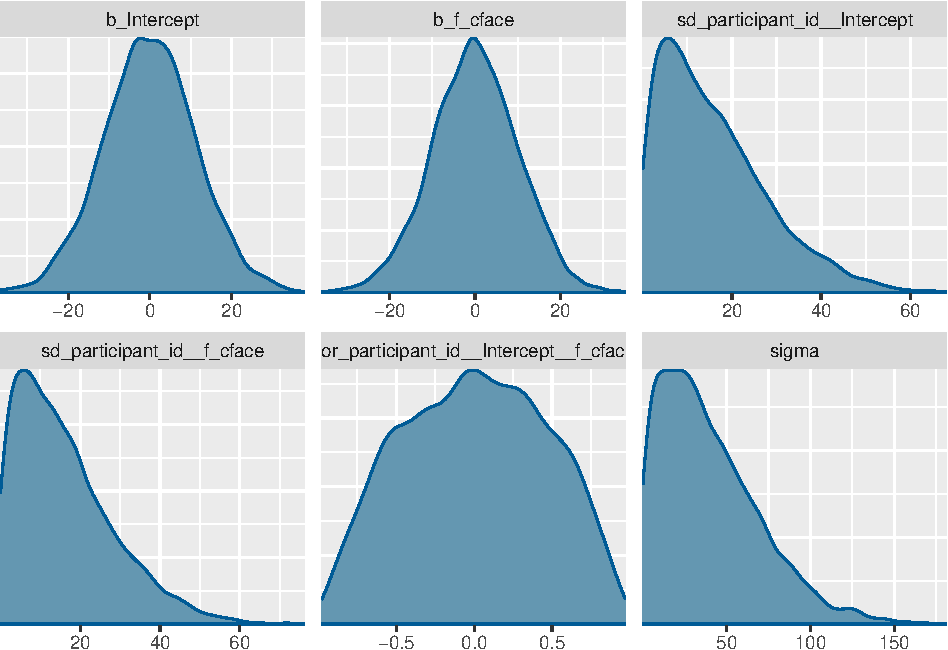
\includegraphics{bachelor_thesis_files/figure-latex/prior-model-plot-1.pdf}
\caption{\label{fig:prior-model-plot}Posterior distributions of the parameters of the prior predictive model}
\end{figure}

However, it can be difficult to visualize how an actual data set with these priors would look like. This is why we additionally look at samples drawn from the prior predictive model. These samples represent how the model predicts possible data sets to look like. With the \texttt{pp\_check} function, we can visualize histograms of these samples. The \texttt{prefix} ``ppd'' specifies, that we are performing prior predictive checks and do not want the original data set to be shown alongside the sample data sets. Already comparing the samples with our actual data might bias us in a certain direction. As we have seen in Sec. 2.4, we would assume our data set to be approximately normally distributed around zero, not exceeding -100 \(\mu V\) and 100 \(\mu V\). For the standard distribution we used a very vague prior, so we would assume some variance here. And this is what we are actually seeing in Fig. \ref{fig:prior-predictive}. We can use the \texttt{pp\_check} function to create these histograms from possible samples of our prior predictive model. The bounds of our samples sometimes exceed the \(+/-\) 100 \(\mu V\) we would expect, but, as we usually want our priors to be a bit wider than our assumptions, this does not pose a problem. The sd of our posterior samples varies substantially like we expected. Unfortunately, the lack of previous EEG experiments using Bayesian methods makes it difficult to determine a good prior for \(\sigma\). In such a case, using a wider prior is usually a good option to not introduce any bias. In summary, our predictive samples seem to match our expectations after prior elicitation.



\begin{Shaded}
\begin{Highlighting}[]
\FunctionTok{pp\_check}\NormalTok{(mod\_ppc, }\AttributeTok{ndraws =} \DecValTok{12}\NormalTok{, }\AttributeTok{type =} \StringTok{"hist"}\NormalTok{, }\AttributeTok{prefix =} \FunctionTok{c}\NormalTok{(}\StringTok{"ppd"}\NormalTok{))}
\end{Highlighting}
\end{Shaded}

\begin{figure}
\centering
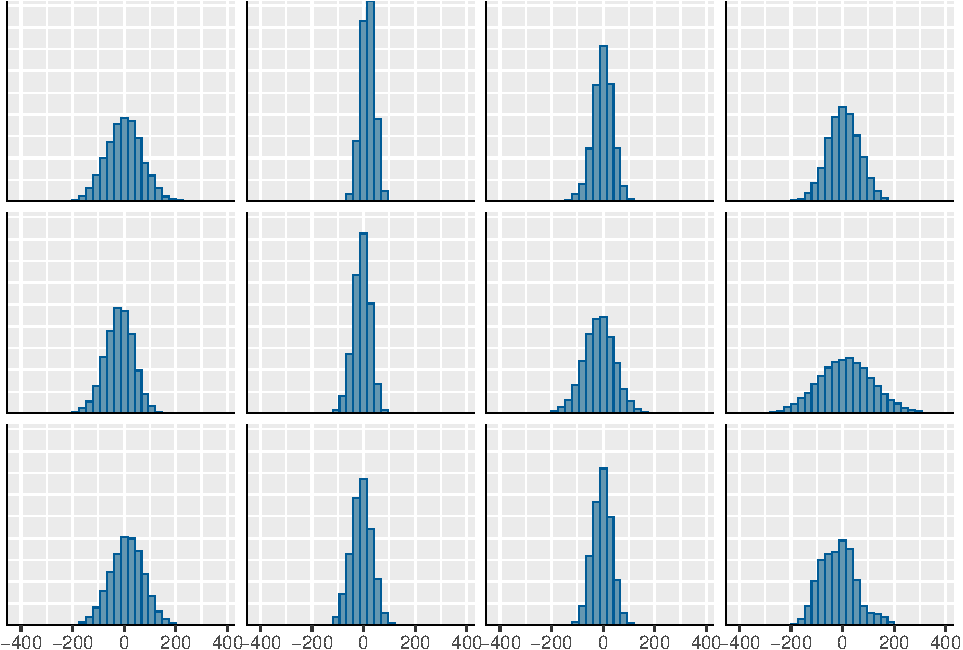
\includegraphics{bachelor_thesis_files/figure-latex/prior-predictive-1.pdf}
\caption{\label{fig:prior-predictive}Sample data sets drawn from the prior predictive model}
\end{figure}

\subsection{Sampling and Convergence}\label{sampling-and-convergence}

For the estimation of the model parameters we need to work out the posterior distribution of our model. However, in most cases the marginal likelihood cannot be computed analytically. Therefore we have to rely on sampling to compute the posterior distribution. With enough samples we will get a good approximation of the posterior. When performing the analysis of Bayesian models with Stan (Team, 2024) or an interface of it, like brms (Bürkner, 2018), the sampling is done using an algorithm called Markov Chain Monte Carlo or, more specifically, Hamiltonian Monte Carlo (Carpenter et al., 2017). MCMC draws sample data sets out of the high dimensional parameter space created by the prior and the likelihood in a way that maps (or reflects??) the posterior distribution. These samples then act as a simulation of the posterior and allow us to extract the distributions of the parameters important to us. This process is usually done several times in different so called chains. The brms package uses four chains per default which follows the recommendation by Vehtari et al. (2021). Each chain undergoes the sampling process independently and the results are then combined. Because the starting point of each chain is picked at random and the algorithm might need some iterations to get to the region of interest, the first iterations are usually treated as a warm-up phase and discarded afterwards. The remaining samples are then treated as the new posterior distribution. The default number of iterations in brms is usually a good start, but we will also see situations in which more iterations are necessary. For a conceptual introduction to MCMC algorithms see Betancourt (2018).

In infinite time this algorithm would always lead to the correct posterior distribution (Roy, 2020). But of course we only have limited time resources. That is why we need to check whether the algorithm converged properly in the amount of iterations we set. We can do so by looking at some convergence criteria. The most commonly used convergence diagnostics are \(\hat{R}\) and the effective sample sizes (Vehtari et al., 2021). Roughly speaking, the \(\hat{R}\) compares the between- and within-chain variance. If the variance of all the chains put together is greater than the variance of one single chain, we assume the sampling has not worked properly. Ideally, every \(\hat{R}\) should be 1, but a good threshold seems to be that \(\hat{R}\) should not be greater than 1.01 (Vehtari et al., 2021). The effective sample size (ESS) reflects the number of independent samples that would contain the same amount of information as the set of correlated samples we get after running the MCMC algorithm (Roy, 2020). We aim for as many effective samples as possible, but at least 400 for every parameter (Vehtari et al., 2021).

The summary of the \texttt{brm}-model gives us some information on the convergence of our model. If the model did not converge properly we also get a warning from Stan. The estimated \(\hat{R}\) can be found under \texttt{Rhat} and the effective sample sizes under \texttt{Bulk\_ESS} for the major part of the posterior distribution and \texttt{Tail\_ESS} for the tails. As we can see in the output of the model from section 2.3 it converged nicely. All the \(\hat{R}\) are smaller or equal to 1.01 and we have an ESS of at least 568 for every parameter. The trace plot (see Fig. \ref{fig:plot-blmm-caption}) of the model also look like we would expect, hoverung equally around the mean of each distribution.

If the sampling did not work properly there are several options to address this. First, we should check if the model is properly defined. Then, we can either use more informative (smaller) priors to constrain the sampling space or increase the number of iterations. Having said that, small deviations from the recommendations (e.g.~if the \texttt{Tail\_ESS} is only 370 for one parameter) are usually not a problem and the model fit should always be looked at as a whole.

\subsection{Posterior Predictive Checks}\label{posterior-predictive-checks}

After computing the complete model and confirming that it converged properly, we can take look at the posterior distribution to determine its descriptive adequacy (Shiffrin et al., 2008). We want to determine if the data predicted by the model is reasonable. This is usually done via posterior predictive checks. In Sec. 2.5 we have seen, that we can draw samples from the posterior distribution of the model. We now want to assess the model's ability to predict data sets similar to our own. Although this can not be seen as good evidence for the model, an inadequacy in properly predicting similar data sets strongly speaks against the model (Shiffrin et al., 2008). Posterior predictive checks can give a first impression of the model predictions, but it should only be seen as a sanity check (Nicenboim et al., n.d.). For model comparison different criteria should be used to assess the performance of a model {[}e.g. Roberts and Pashler (2000); xxx{]}.

To perform posterior predictive checks we can again use the \texttt{pp\_check} function. Looking at Fig \ref{fig:posterior-check-blmm-hist}, the samples indeed look very similar to our observed data. The only difference seems to ba a slightly smaller standard deviation, the actual data set has a higher peak and a narrower distribution. Apart from that the model predicts data sets closely related to the observed data. For EEG experiments this will usually be the case, because we have so many data points and the prior plays a smaller role in the posterior predictive distribution.



\begin{Shaded}
\begin{Highlighting}[]
\FunctionTok{pp\_check}\NormalTok{(mod\_blmm, }\AttributeTok{ndraws =} \DecValTok{11}\NormalTok{, }\AttributeTok{type =} \StringTok{"hist"}\NormalTok{)}
\end{Highlighting}
\end{Shaded}

\begin{figure}
\centering
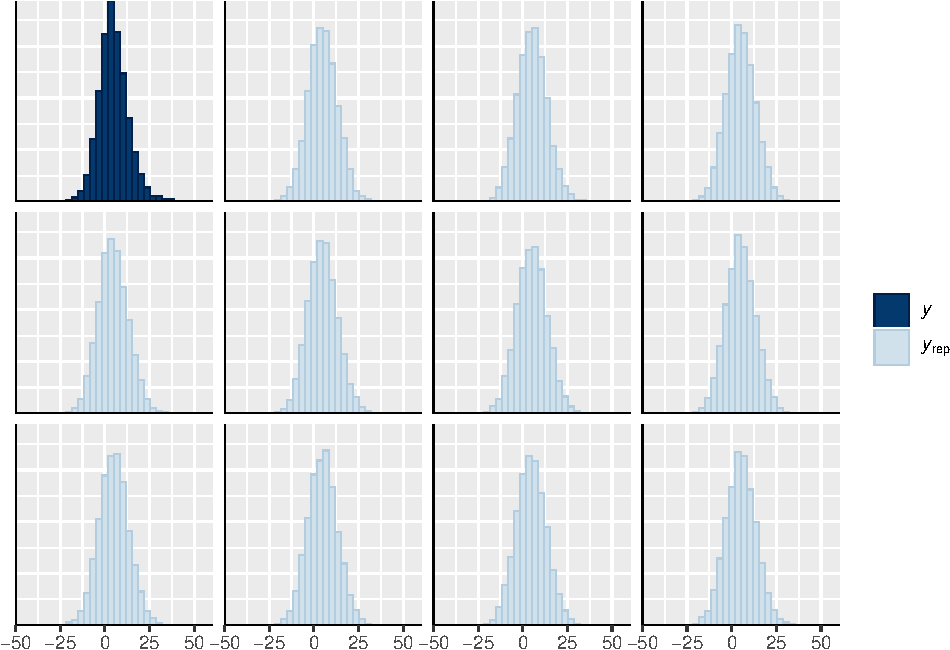
\includegraphics{bachelor_thesis_files/figure-latex/posterior-check-blmm-hist-1.pdf}
\caption{\label{fig:posterior-check-blmm-hist}Histograms of the original data set and of samples drawn from the posterior predictive distribution}
\end{figure}

When specifying the \texttt{type} of the \texttt{pp\_check} function as ``dens-overlay'' we can directly compare the distributions of our predicted samples with the actual data set. This emphasize the small difference between the actual data and the predicted samples. The model does not cover all the information contained in the data. In the next section we will introduce a new model to account for this difference.



\begin{Shaded}
\begin{Highlighting}[]
\FunctionTok{pp\_check}\NormalTok{(mod\_blmm, }\AttributeTok{ndraws =} \DecValTok{100}\NormalTok{, }\AttributeTok{type =} \StringTok{"dens\_overlay"}\NormalTok{)}
\end{Highlighting}
\end{Shaded}

\begin{figure}
\centering
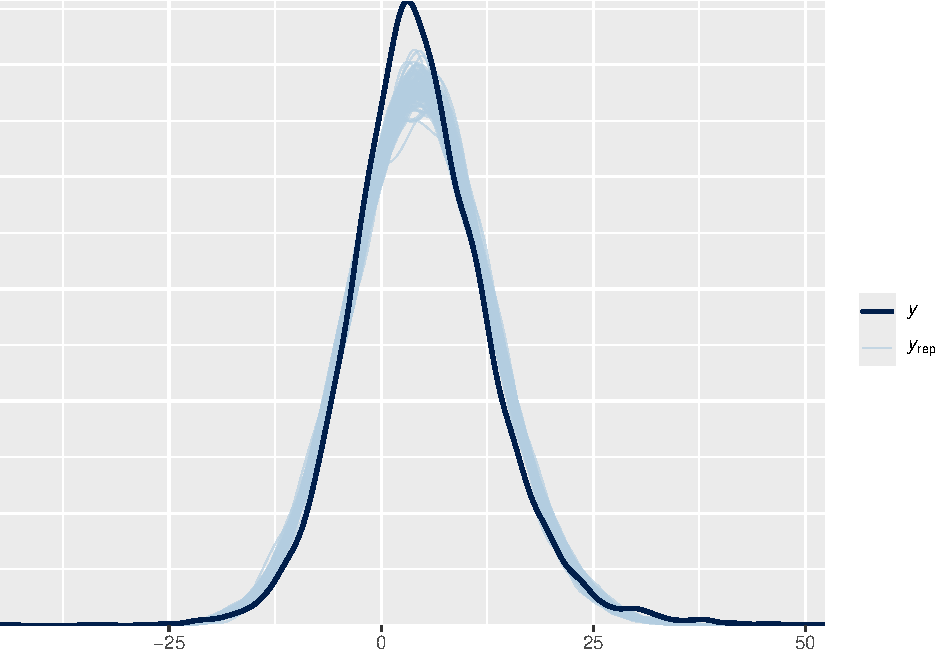
\includegraphics{bachelor_thesis_files/figure-latex/posterior-check-blmm-density-1.pdf}
\caption{\label{fig:posterior-check-blmm-density}Density plot of the original data set and of samples drawn from the posterior predictive distribution}
\end{figure}

\subsection{Distributional Regression}\label{distributional-regression}

As we have seen in the previous section, there is a part of the signal distribution that the model cannot account for. This could be explained by a high variance of noise levels between participants (Nicenboim et al., n.d.). In ERP studies the level of impedance between skin and electrodes has a significant effect on the amount of noise in the data (Picton et al., 2000). Since the impedance is depending on the skin tissue of each subject the amount of noise might be varying a lot. We can check this hypothesis with the following code that shows posterior samples grouped by participant.



\begin{Shaded}
\begin{Highlighting}[]
\CommentTok{\# Posterior predictive check by participant}
\FunctionTok{pp\_check}\NormalTok{(mod\_blmm, }
         \AttributeTok{type =} \StringTok{"dens\_overlay\_grouped"}\NormalTok{,}
         \AttributeTok{ndraws =} \DecValTok{100}\NormalTok{,}
         \AttributeTok{group =} \StringTok{"participant\_id"}\NormalTok{)}
\end{Highlighting}
\end{Shaded}

\begin{figure}
\centering
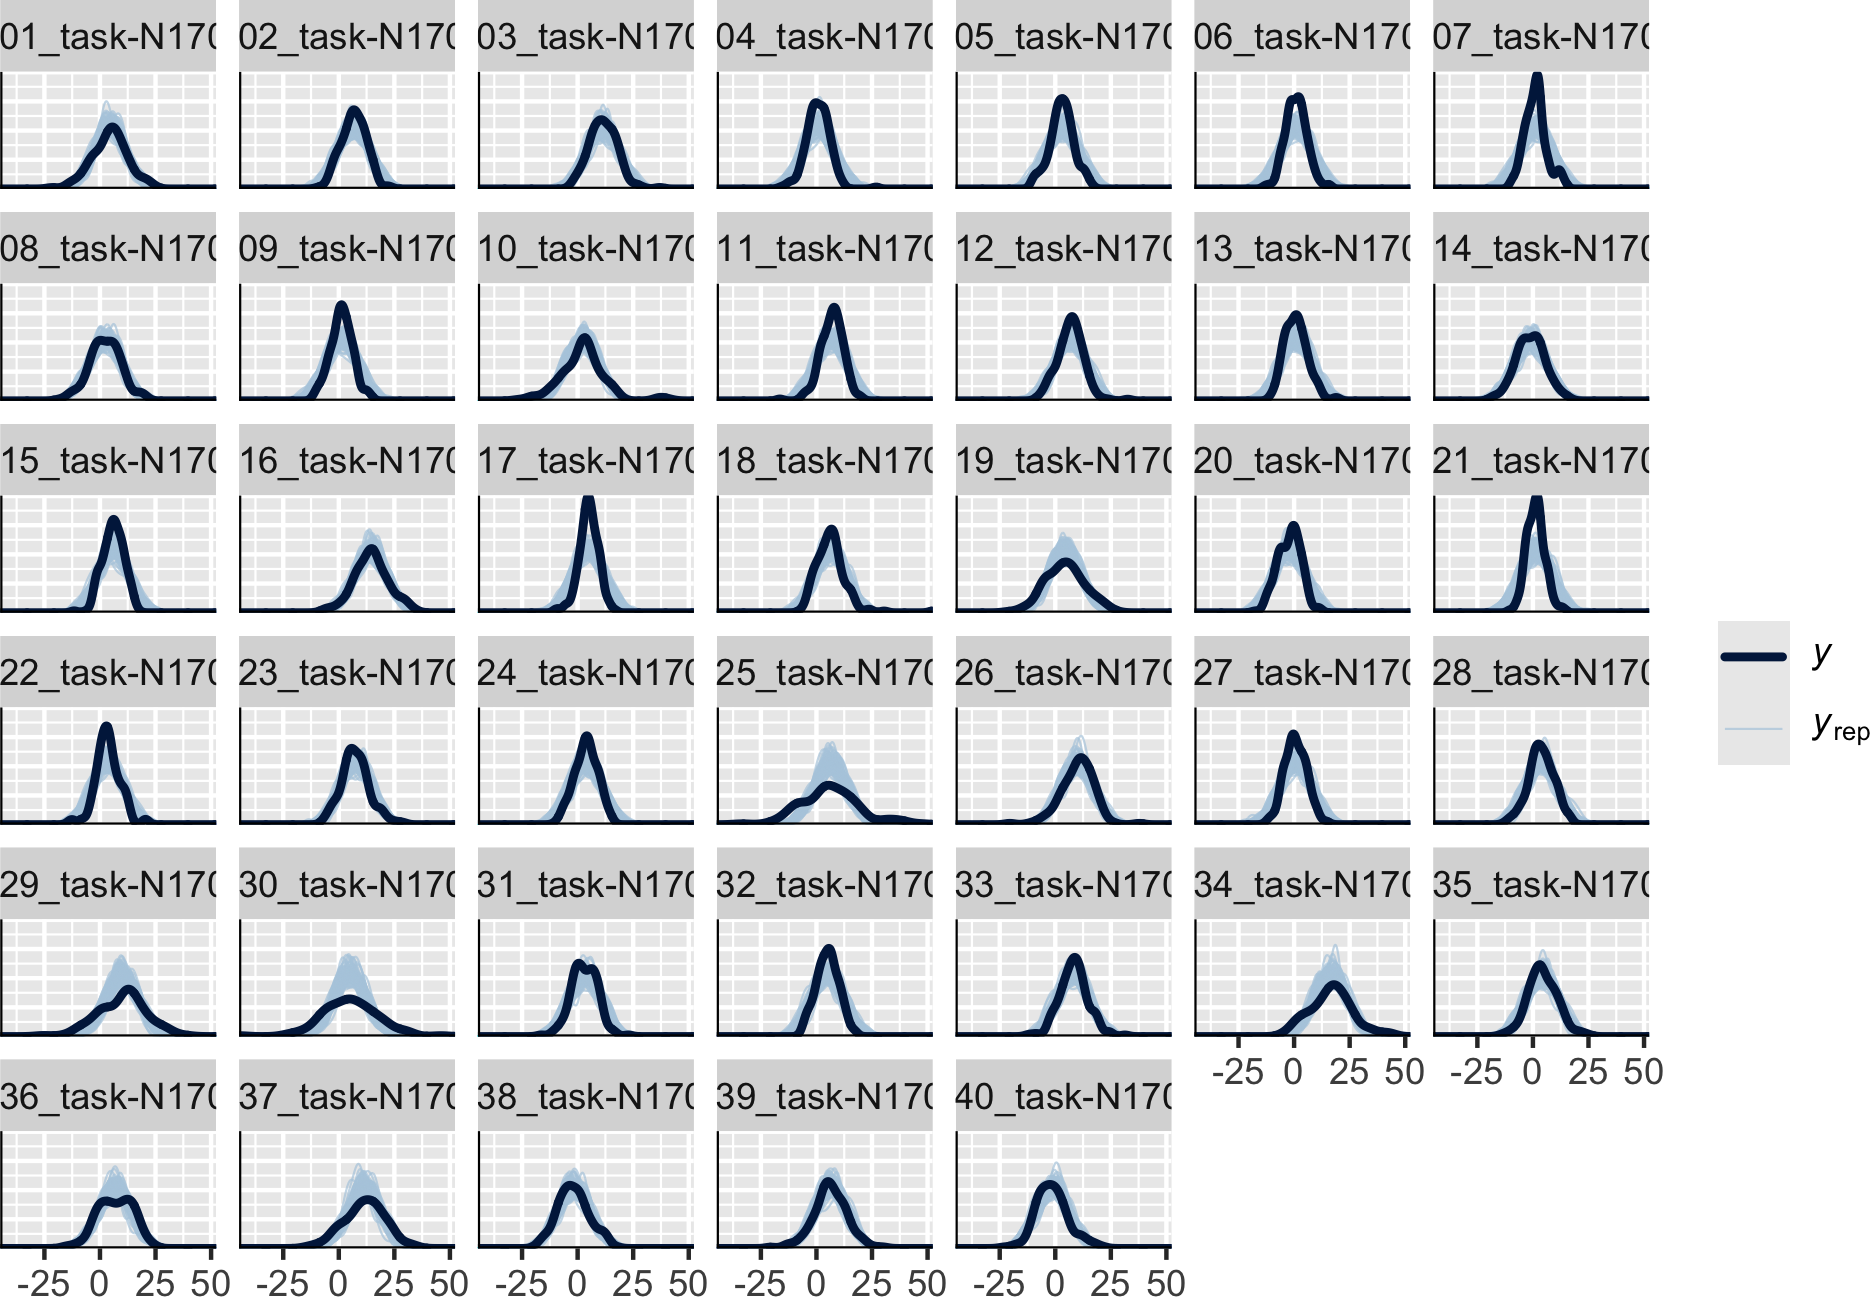
\includegraphics{bachelor_thesis_files/figure-latex/sigma-variance-1.pdf}
\caption{\label{fig:sigma-variance}Predicted distributions of the N170 signal data grouped by participant}
\end{figure}



\begin{Shaded}
\begin{Highlighting}[]
\FunctionTok{pp\_check}\NormalTok{(mod\_blmm,}
         \AttributeTok{type =} \StringTok{"stat\_grouped"}\NormalTok{,}
         \AttributeTok{ndraws =} \DecValTok{1000}\NormalTok{,}
         \AttributeTok{group =} \StringTok{"participant\_id"}\NormalTok{,}
         \AttributeTok{stat =} \StringTok{"sd"}\NormalTok{,}
         \AttributeTok{facet\_args =} \FunctionTok{list}\NormalTok{(}\AttributeTok{scales =} \StringTok{"fixed"}\NormalTok{))}
\end{Highlighting}
\end{Shaded}

\begin{figure}
\centering
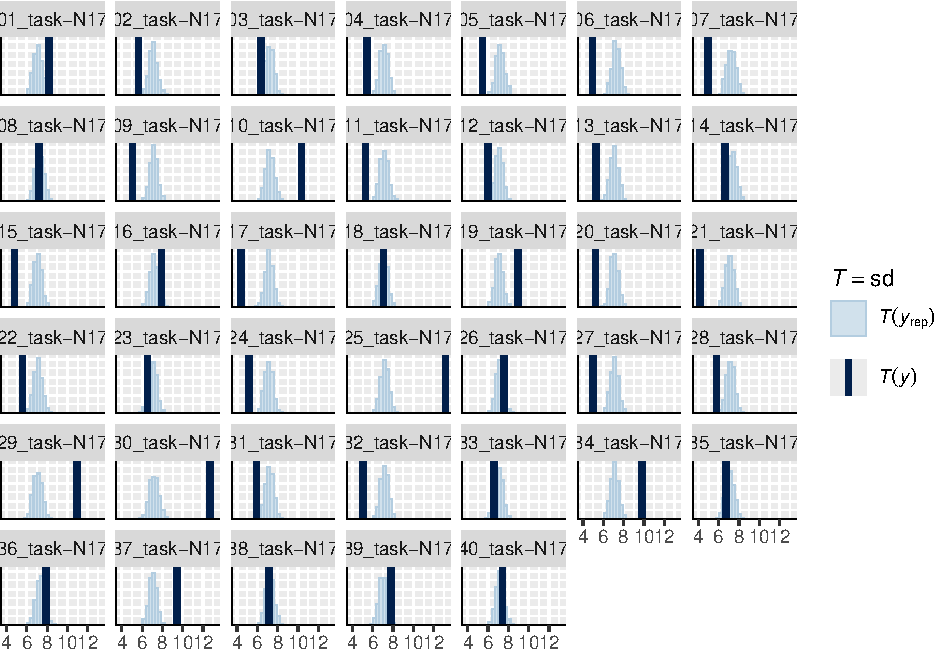
\includegraphics{bachelor_thesis_files/figure-latex/sigma-variance-sd-1.pdf}
\caption{\label{fig:sigma-variance-sd}Predicted standard deviations of the N170 signal data grouped by participant}
\end{figure}

As we can see in Fig. \ref{fig:sigma-variance} there are indeed highly varying noise levels between the participants that our current model does not capture. By assuming the same within person variance \(\sigma\) for all participants we might be misfitting participants with significantly lower or higher \(\sigma\) (Nicenboim et al., n.d.). To account for these differences we will look at a new kind of statistical model.

Usually, models in psychology only contemplate differences regarding the mean. Whether we look at differences between groups, experimental conditions or individuals, difference is commonly defined as difference in mean. Differences in scale or shape are just regarded a nuisance because they might violate the assumptions of our models (e.g.~the homoscedasticity assumption in linear models). In distributional models, also called generalized additive models for location, scale and shape (GAMLSS), the entire distribution is modeled for each group or individual separately, therefore incorporating any differences in scale or shape into the model (Klein, 2024). With these models differences in noise levels could be modeled instead of being ignored. Fortunately, the brms package allows for an easy extension to distributional regression Bürkner (2024). This emphasizes the flexibility of the Bayesian framework, enabling us to conveniently adapt to the data at hand. The computational back-end using modern MCMC algorithms is also powerful enough to estimate these much more complex models (Bürkner, 2024). See Kneib et al. (2023) for a review of distributional regression approaches.

\subsubsection{Mathematical Model and Implementation in R}\label{mathematical-model-and-implementation-in-r-1}

In our case we assume that the shape of the signal remains a normal distribution for every participant, only the variance of this normal distribution can differ between participants. We thereby introduce the hierarchical structure of our data into variance component as well.

The formal model will change in a way that the single trial averages will now have a subject-specific \(\sigma\). The \(\sigma\) is hence dependent on what person the trial belongs to but does not differ for the experimental condition. We do not expect the condition of faces vs.~cars to influence the signal variance. We exponentiate \(\sigma\) so that it cannot become negative even with negative adjustments (Nicenboim et al., n.d.). Equation \eqref{eq:dist-reg} shows our new model.

\begin{equation}
\begin{split}
& y_{ij} \sim N(\beta_0 + u_{j,1} + X_{ij}(\beta_1 + u_{j,2}), \enspace \sigma_j) \\
& With \enspace \sigma_j = exp(\sigma_{\beta_0} + \sigma_{u_j})
\end{split}
\label{eq:dist-reg}
\end{equation}

We also need to add priors to the new parameters. Since no ERP studies have used distributional models so far we, unfortunately, have very little prior knowledge on how the parameters behave. Therefore, we first remained with the previous prior for the intercept of the sigma (now as log(50) because it will be exponentiated afterwards). For the variance component of sigma we chose a rather uninformative prior.

\begin{equation}
\begin{split}
& \sigma_{\beta_0} \sim N(0, log(50)) \\
& \sigma_{u_j} \sim N(0, \tau_{\sigma_u}) \\
& \tau_{\sigma_u} \sim N_{+}(0,5)
\end{split}
\label{eq:prior-dist}
\end{equation}

By performing a sensitivity analysis using prior predictive checks we have then verified if our chosen priors were actually sensible. This allows us to see that the priors in Eq. \eqref{eq:prior-dist} are too broad and the means of the signal averages are too spread out. We will not look at the prior predictive checks in detail here because the concept remains the same, further details can be found in the corresponding script. Following the sensitivity analysis, we have then decided on the following prior, denoted by \texttt{dpar\ =\ sigma} (distributional parameter).

\begin{Shaded}
\begin{Highlighting}[]
\CommentTok{\# Prior for distributional regression}
\NormalTok{prior\_dist }\OtherTok{\textless{}{-}} \FunctionTok{c}\NormalTok{(}
  \FunctionTok{prior}\NormalTok{(}\FunctionTok{normal}\NormalTok{(}\DecValTok{0}\NormalTok{, }\DecValTok{10}\NormalTok{), }\AttributeTok{class =}\NormalTok{ Intercept), }
  \FunctionTok{prior}\NormalTok{(}\FunctionTok{normal}\NormalTok{(}\DecValTok{0}\NormalTok{, }\DecValTok{10}\NormalTok{), }\AttributeTok{class =}\NormalTok{ b, }\AttributeTok{coef =}\NormalTok{ f\_cface),}
  \CommentTok{\# intercept of sigma}
  \FunctionTok{prior}\NormalTok{(}\FunctionTok{normal}\NormalTok{(}\DecValTok{0}\NormalTok{, }\FunctionTok{log}\NormalTok{(}\DecValTok{3}\NormalTok{)), }\AttributeTok{class =}\NormalTok{ Intercept, }\AttributeTok{dpar =}\NormalTok{ sigma), }
  \CommentTok{\# variance component of sigma}
  \FunctionTok{prior}\NormalTok{(}\FunctionTok{normal}\NormalTok{(}\DecValTok{0}\NormalTok{, }\DecValTok{1}\NormalTok{), }\AttributeTok{class =}\NormalTok{ sd, }
        \AttributeTok{group =}\NormalTok{ participant\_id, }\AttributeTok{dpar =}\NormalTok{ sigma), }
  \FunctionTok{prior}\NormalTok{(}\FunctionTok{normal}\NormalTok{(}\DecValTok{0}\NormalTok{, }\DecValTok{20}\NormalTok{), }\AttributeTok{class =}\NormalTok{ sd, }\AttributeTok{coef =}\NormalTok{ Intercept, }
        \AttributeTok{group =}\NormalTok{ participant\_id),  }
  \FunctionTok{prior}\NormalTok{(}\FunctionTok{normal}\NormalTok{(}\DecValTok{0}\NormalTok{, }\DecValTok{20}\NormalTok{), }\AttributeTok{class =}\NormalTok{ sd, }\AttributeTok{coef =}\NormalTok{ f\_cface, }
        \AttributeTok{group =}\NormalTok{ participant\_id), }
  \FunctionTok{prior}\NormalTok{(}\FunctionTok{lkj}\NormalTok{(}\DecValTok{2}\NormalTok{), }\AttributeTok{class =}\NormalTok{ cor, }\AttributeTok{group =}\NormalTok{ participant\_id)}
\NormalTok{  ) }
\end{Highlighting}
\end{Shaded}

To fit our model in brms we need to use the function \texttt{brmsformula} (or its alias \texttt{bf}) (Bürkner, 2024). This function allows as to extend the current formula to a distributional regression, applying the hierarchical nature of the data to any parameter. The first part inside the \texttt{bf} function stays the same, the second part, after the comma, allows us to specify the structure of the distributional part. As mentioned before, in our case the scale (sigma) of the distribution will only depend on the subject, we are therefore adding a random effect here. We fit the model with increased iterations (\texttt{iter}) due to the higher complexity of the model (a new parameter must be fitted for every participant).

\begin{Shaded}
\begin{Highlighting}[]
\CommentTok{\# Distributional regression model }
\NormalTok{mod\_dist }\OtherTok{\textless{}{-}} \FunctionTok{brm}\NormalTok{(}\FunctionTok{bf}\NormalTok{(N170 }\SpecialCharTok{\textasciitilde{}} \DecValTok{1} \SpecialCharTok{+}\NormalTok{ f\_c }\SpecialCharTok{+}\NormalTok{ (}\DecValTok{1} \SpecialCharTok{+}\NormalTok{ f\_c }\SpecialCharTok{|}\NormalTok{ participant\_id), }
\NormalTok{                   sigma }\SpecialCharTok{\textasciitilde{}} \DecValTok{1} \SpecialCharTok{+}\NormalTok{ (}\DecValTok{1} \SpecialCharTok{|}\NormalTok{ participant\_id)), }
                \AttributeTok{data =}\NormalTok{ trials\_cond, }
                \AttributeTok{prior =}\NormalTok{ prior\_dist,}
                \AttributeTok{family =} \FunctionTok{gaussian}\NormalTok{(),}
                \AttributeTok{iter =} \DecValTok{4000}\NormalTok{,}
                \AttributeTok{warmup =} \DecValTok{1000}\NormalTok{,}
                \AttributeTok{cores =} \DecValTok{4}\NormalTok{) }
\end{Highlighting}
\end{Shaded}

\subsubsection{Results}\label{results-2}

As before, we will first take a look at the output of the \texttt{summary} function to get an overview of our fitted model.



\footnotesize

\begin{verbatim}
##  Family: gaussian 
##   Links: mu = identity; sigma = log 
## Formula: N170 ~ 1 + f_c + (1 + f_c | participant_id) 
##          sigma ~ 1 + (1 | participant_id)
##    Data: trials_cond (Number of observations: 6224) 
##   Draws: 4 chains, each with iter = 4000; warmup = 1000; thin = 1;
##          total post-warmup draws = 12000
## 
## Multilevel Hyperparameters:
## ~participant_id (Number of levels: 40) 
##                        Estimate Est.Error l-95% CI u-95% CI Rhat Bulk_ESS
## sd(Intercept)              4.33      0.55     3.40     5.53 1.00     1530
## sd(f_cface)                1.55      0.28     1.05     2.14 1.00     4296
## sd(sigma_Intercept)        0.29      0.04     0.23     0.38 1.00     1619
## cor(Intercept,f_cface)     0.06      0.19    -0.32     0.43 1.00     4789
##                        Tail_ESS
## sd(Intercept)              2810
## sd(f_cface)                7224
## sd(sigma_Intercept)        2700
## cor(Intercept,f_cface)     6411
## 
## Regression Coefficients:
##                 Estimate Est.Error l-95% CI u-95% CI Rhat Bulk_ESS Tail_ESS
## Intercept           5.65      0.73     4.22     7.11 1.01      795     1696
## sigma_Intercept     1.87      0.05     1.78     1.96 1.00     1373     2452
## f_cface            -1.76      0.31    -2.37    -1.16 1.00     4064     6074
## 
## Draws were sampled using sampling(NUTS). For each parameter, Bulk_ESS
## and Tail_ESS are effective sample size measures, and Rhat is the potential
## scale reduction factor on split chains (at convergence, Rhat = 1).
\end{verbatim}

\normalsize

Notice that the estimate of the main effect, the difference between the perception of faces and cars in the N170, remains almost the same with \(b_1\) = -1.76 compared to \(b_1\) = -1.76 in the standard BLMM. The same goes for the intercept which also changes only slightly from \(b_0\) = 5.65 to \(b_0\) = 5.67 in the previous model. The two new parameters in our distibutional model are referred to as \texttt{sd(sigma\_intercept)} for the variance component of sigma and \texttt{sigma\_Intercept} for the intercept of the sigma.

The model also seems to have converged nicely, as all \(\hat{R}\) are under \(1.01\) and the ESS are at a minimum of 793.

Nonetheless, by performing a posterior predictive check it becomes clear that the new model can fit our data better than the old one (see Fig. \ref{fig:posterior-check-dist}), fitting every part of the distribution. Accounting for the differences in noise level between participants seems to have made a difference for the model fit at least on a visual level. This leads us to expect an improved prediction capacity of the model. In the next section we will look at a way to quantify this improvement.



\begin{figure}
\centering
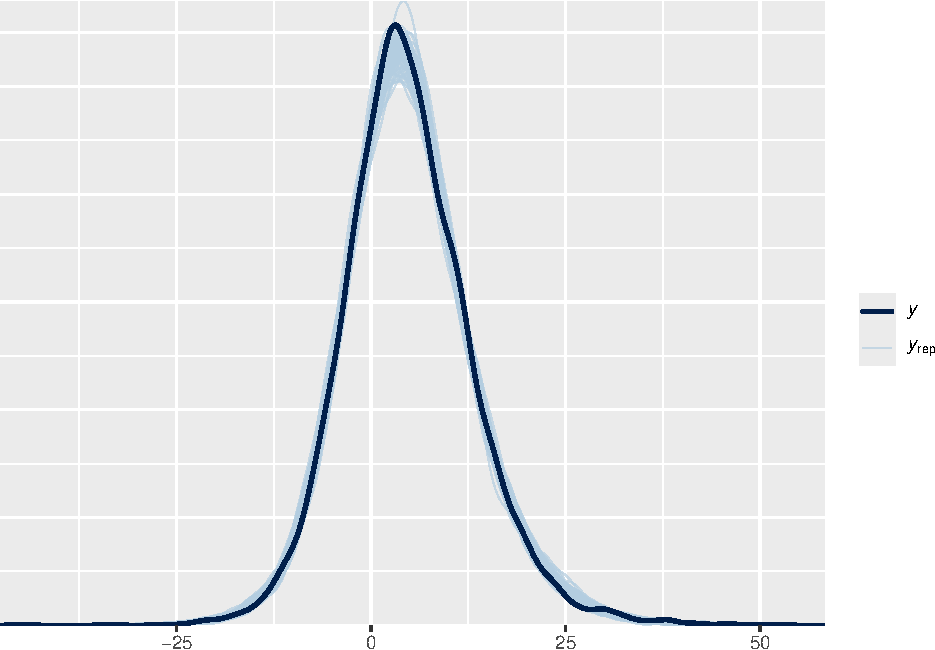
\includegraphics{bachelor_thesis_files/figure-latex/posterior-check-dist-1.pdf}
\caption{\label{fig:posterior-check-dist}Overlay of densities from posterior sample from the distributional model}
\end{figure}

\subsection{Hypothesis Testing}\label{hypothesis-testing}

A primary goal of experiments in cognitive psychology is to test a certain theory. In frequentist analyses this is usually done using null hypothesis significance testing (NHST). NHST is a way of deciding if one theory accounts better for the observed data than another. Usually,
When using NHST researchers will not only want to know the
In Bayesian statistics this approach is often criticized
Because it is standard part of the frequentist framework and almost always reported in ERP studies, the following sections will concentrate on two different approaches to NHST in Bayesian statistics, Bayes factors and cross validation. Both come with distinct advantages and drawbacks that will also be discussed. However, as mentioned before, most Bayesian statisticians would advise against dichotomous decisions and therefore these methods should always be regarded critically.

generalization only within range of the observed data

``A model that's closest to the true generating data process is not guaranteed to produce the best (prior or posterior) predictions, and a model with a clearly wrong generating data process is not guaranteed to produce poor (prior or posterior) predictions'' Nicenboim et al. (n.d.)

precision of the data -\textgreater{} effect on comparison (wie viele Datenpunkte brauche ich -\textgreater{} Power???)

Important to note, that credible intervals should not be used to reject or accept a null hypothesis (Wagenmakers et al. (2019)).

\subsection{Bayes Factors}\label{bayes-factors}

As mentioned above Bayes Factors are one way to test hypothesis in the Bayesian framework. The BF assess how well the entire model (prior and likelihood) is able to explain the observed data set (Nicenboim et al., n.d.).

highly sensitive to priors

bridge sampling

this approach to model comparison could also be seen as not ``truly''
Bayesian in the sense that they rely on a point estimate of the parameter rather than incorporating
the entire posterior.

collecting evidence for null hypothesis -\textgreater{} pro Bayes

interpretation that we often want in freq -\textgreater{} pro Bayes

\subsubsection{Sensitivity Analysis}\label{sensitivity-analysis}



\subsection{Cross Validation}\label{cross-validation}

The other approach to compare Bayesian models is cross validation. In contrast to the BF, in cross validation the model is fit only to a subset of the data (training data). The resulting posterior distribution is then used to predict the held-out (or validation) data and the accuracy of the prediction is assessed. This process is repeated several times, until every subset of a partition was left out once. In the following, we will use leave-one-out cross validation {[}LOO; e.g., Gelman et al. (2014); Vehtari et al. (2017){]}, where the validation data consists only of one data point. Cross validation attempts to assess how our model deals with new data and if we can generalize to out-of-sample data. Of course the validation data are not actually new, as they were collected with the rest of the data set (Nicenboim et al., n.d.). This approach is less dependent on the prior distribution, especially with the amount of data seen in ERP studies forming the likelihood.

To quantify the accuracy of the prediction, we will use an estimator called \emph{expected log pointwise predictive density} (\(elpd\)). For each held-out data point the predictive density, given the model and the training data, is calculated. The elpd is obtained by summing over the log of these predictive densities (Gronau \& Wagenmakers, 2019). To compare two models the difference between the elpd's is computed and the magnitude of this difference is assessed. We will not worry about the further mathematicel specifics here, see Gelman et al. (2014) and Nicenboim et al. (n.d.) for a detailed introduction to LOO.

For the computation we use the \texttt{loo} function from the brms package, which builds on the loo package as a backend (Vehtari, Gabry, et al., 2024) It uses Pareto smoothed importance sampling {[}PSIS; Vehtari, Simpson, et al. (2024){]} to compute the \(elpd\). Importance sampling allows to estimate sample from the posterior distribution after removal of one data point without having to re-fit the entire model every time (Vehtari et al., 2017). PSIS is a newer, more stable version of this algorithm providing more reliable and accurate estimates (Vehtari, Simpson, et al., 2024).

The implementation is very straightforward. We first need to calculate the elpd for each model we want to compare. In our case again, that means one model with the fixed effect of faces vs.~cars and one null model without this effect. Unlike with BF, we don't need to increase the iterations because the estimation of the \(elpd\) depends mainly on the number of observations and not the number of samples (Nicenboim et al., n.d.). We only need to set up the null model as in Section 2.10 and then use the \texttt{loo} function for every model. The \texttt{loo} function not only gives us the \texttt{elpd\_loo}, the sum of pointwise predictive accuracy (here a less negative number indicates a better prediction). But also the effective number of parameters \texttt{p\_loo}, an estimate of model complexity, and the LOO information criterion \texttt{looic}, which is just \texttt{-2*elpd\_loo}. Additionally, the function will output some diagnostics. We will not discuss them here, but in general it is important for a reliable estimation that the Pareto k estimates are small enough (under .7) (see Vehtari et al., 2017). After computing the \(elpd\) we can use the \texttt{loo\_compare} function to compare the models. \texttt{loo\_compare} computes the difference between the \(elpd\) of the two models (\texttt{elpd\_diff}) as well as the standard error of this difference (\texttt{se\_diff}).

\begin{Shaded}
\begin{Highlighting}[]
\CommentTok{\# Computing the elpd for the standard correlation model}
\NormalTok{loo\_blmm\_1 }\OtherTok{\textless{}{-}} \FunctionTok{loo}\NormalTok{(mod\_blmm)}

\CommentTok{\# Computing the elpd for the null model}
\NormalTok{loo\_blmm\_0 }\OtherTok{\textless{}{-}} \FunctionTok{loo}\NormalTok{(mod\_blmm\_0)}
\CommentTok{\#apa\_table(loo\_blmm\_0["estimates"])}

\CommentTok{\# Comparing the models}
\NormalTok{loo\_comparison\_blmm }\OtherTok{\textless{}{-}} \FunctionTok{loo\_compare}\NormalTok{(loo\_blmm\_1, loo\_blmm\_0)}
\end{Highlighting}
\end{Shaded}

\begin{table}[tbp]

\begin{center}
\begin{threeparttable}

\caption{\label{tab:loo-blmm-table}}

\begin{tabular}{lllllllll}
\toprule
 & \multicolumn{1}{c}{elpd\_diff} & \multicolumn{1}{c}{se\_diff} & \multicolumn{1}{c}{elpd\_loo} & \multicolumn{1}{c}{se\_elpd\_loo} & \multicolumn{1}{c}{p\_loo} & \multicolumn{1}{c}{se\_p\_loo} & \multicolumn{1}{c}{looic} & \multicolumn{1}{c}{se\_looic}\\
\midrule
mod\_blmm & 0.00 & 0.00 & -21,033.82 & 85.91 & 69.42 & 2.11 & 42,067.64 & 171.82\\
mod\_blmm\_0 & -2.66 & 2.69 & -21,036.48 & 85.89 & 74.88 & 2.25 & 42,072.96 & 171.78\\
\bottomrule
\end{tabular}

\end{threeparttable}
\end{center}

\end{table}

\begin{table}[tbp]

\begin{center}
\begin{threeparttable}

\caption{\label{tab:loo-dist-table}Comparison of the linear and null distributional model usind LOO}

\begin{tabular}{lllllllll}
\toprule
 & \multicolumn{1}{c}{elpd\_diff} & \multicolumn{1}{c}{se\_diff} & \multicolumn{1}{c}{elpd\_loo} & \multicolumn{1}{c}{se\_elpd\_loo} & \multicolumn{1}{c}{p\_loo} & \multicolumn{1}{c}{se\_p\_loo} & \multicolumn{1}{c}{looic} & \multicolumn{1}{c}{se\_looic}\\
\midrule
mod\_dist & 0.00 & 0.00 & -20,516.62 & 72.36 & 120.80 & 7.61 & 41,033.23 & 144.72\\
mod\_dist\_0 & -1.72 & 2.52 & -20,518.33 & 72.29 & 125.46 & 7.44 & 41,036.67 & 144.58\\
\bottomrule
\end{tabular}

\end{threeparttable}
\end{center}

\end{table}

Table \ref{tab:loo-blmm-table} shows the \(elpd\) difference and the se of said difference in the first two columns as well as more detailed information about the models (including \texttt{elpd\_loo}, \texttt{p\_loo} and \texttt{looic}) in the rear columns. An \(elpd\) difference of \(elpd_{diff}\) = -2.70 tells us that the the model with the experimental condition as a predictor has a higher predictive accuracy. Although this supports our initial hypothesis, as the difference is smaller than 4 and also smaller than 2 \(se\), it cannot be interpreted as a meaningful superiority of one model over the other (Nicenboim et al., n.d.).

The same pattern arises in the comparison of the linear und null distributional model. As we can see in Table \ref{tab:loo-dist-table} the \(elpd_{diff}\) of -1.70 is similarly small.

\begin{table}[tbp]

\begin{center}
\begin{threeparttable}

\caption{\label{tab:loo-blmm-dist-table}}

\begin{tabular}{lllllllll}
\toprule
 & \multicolumn{1}{c}{elpd\_diff} & \multicolumn{1}{c}{se\_diff} & \multicolumn{1}{c}{elpd\_loo} & \multicolumn{1}{c}{se\_elpd\_loo} & \multicolumn{1}{c}{p\_loo} & \multicolumn{1}{c}{se\_p\_loo} & \multicolumn{1}{c}{looic} & \multicolumn{1}{c}{se\_looic}\\
\midrule
mod\_dist & 0.00 & 0.00 & -20,516.62 & 72.36 & 120.80 & 7.61 & 41,033.23 & 144.72\\
mod\_blmm & -517.20 & 45.32 & -21,033.82 & 85.91 & 69.42 & 2.11 & 42,067.64 & 171.82\\
\bottomrule
\end{tabular}

\end{threeparttable}
\end{center}

\end{table}

The comparison between the distributional and the standard LMM (see Table \ref{tab:loo-blmm-dist-table}) confirms the strong superiority of the distributional model that we had already seen with the BFs with an \(elpd_{diff}\) of -517.20.

These results

never a whole new subject
small effects
difference to BF
inconsistent

\subsection{Reporting Practices}\label{reporting-practices}

Analyses with BLMMs imply a great amount of researchers degrees of freedom, and thus it is essential to provide enough information on the analysis for others to be able to replicate and evaluate it. Simmons et al. (2011) show impressively what can happen when analyses are not disclosed. Ideally, the entire code (and, if possible, data) should be uploaded in an online repository like the Open Science Framework or GitHub (Epskamp, 2019). This not only provides all the analyses in one place but also solves the problem of having to decide what to report within a possibly limited word count. In addition, if the analyses were conducted in R researchers could consider making it entirely reproducible (see e.g., Brandmaier \& Peikert, 2024; Marwick et al., 2018; Peikert \& Brandmaier, 2019).

Generally, the software used for the analyses should be cited as well as all associated packages with version numbers respectively. Epskamp (2019) even suggests to use a package like renv ((\textbf{R-renv?})) that stores the source code of every package at the point of use and makes later reproducibility much easier. Also, setting a seed for the generation of pseudorandom numbers at the beginning of the analysis helps with more exact reproducibility. The variables (dependent and independent) should be clearly named and explained further if necessary (Kruschke, 2021). It might also be helpful, to explain why one chose a specific method and explain the method and possible benefits if the audience requires it (Kruschke, 2021). Additionally, for different methods different aspects might be reported (e.g.~inclusion criteria for a meta-analysis(Hansen et al., 2022)). We will discuss the primary reporting practices for LMMs and Bayesian methods next.

For frequentist LMMs Meteyard and Davies (2020) provide a comprehensive overview on reporting practices. They recommend to report the equation of the final model as well as the approach used for model selection. Reporting additional models (not only the final one) can also be beneficial (Wagenmakers et al., 2021). Meteyard and Davies (2020) also suggest to provide point estimates, standard error and confidence interval of the fixed effects and all variances of random effects. If p values are used the method to approximate degrees of freedom should be stated (Meteyard \& Davies, 2020).

In Bayesian statistics reporting becomes even more important due to the increased researchers degrees of freedom but also more complicated because among others we are dealing with posterior distributions not only point estimates. Depending on the performed analysis very different things should be reported in papers using Bayesian methods. In the following we will concentrate on the most important aspects for the analyses performed above. Kruschke (2021) gives a more detailed review on Bayesian reporting practices and guidelines to improve reproducibility and quality of Bayesian analyses.

As part of the methods presentation the assumed likelihood function should be explained, the prior distributions should be stated and justified for each parameter and the model should be formally specified (include likelihood and prior) (Kruschke, 2021). For multilevel models, like the ones discussed in this paper, the hierarchical structure should be explained. Kruschke (2021) recommends performing and reporting prior predictive checks (see Section xxx), especially for more informative priors. The performance of the computation (MCMC in our case) should also be reported, here Kruschke (2021) recommends to report a convergence measure, like the \(\hat{R}\) seen above, and a measure for the resolution, this refers to the ESS. Since MCMC algorithms can be quite time-intensive it might be advised to publish the entire MCMC chain. The posterior distributions should be summarized by a measure of central tendency and the credible interval, ideally posterior predictive checks should show that the model mimics the data (Kruschke, 2021). For the hypothesis testing Kruschke (2021) suggests to state the decision procedure/threshold and the observed BF and posterior probabilities or the observed difference in elpd. Finally, the sensitivity analysis should be reported to show if or how the prior influences the posterior and especially if the decisions change under different priors (Kruschke, 2021). Of course, additional analysis might need further reporting and researchers might chose to address some of the points discussed in the appendix or supplementary material.

\section{Discussion}\label{discussion}

\subsection{Advantages and Disadvantages of Bayesian Linear Mixed Models}\label{advantages-and-disadvantages-of-bayesian-linear-mixed-models}

\begin{itemize}
\tightlist
\item
  Advantages: flexibility (as with dist model),
\item
  computational power
\end{itemize}

Vorteile LMM:
- für EEG gut geeignet, da immer enough sample size (many trials per person, subject number per item)

\begin{itemize}
\tightlist
\item
  power analysis should not be needed for classical bayesian, but what about BF
\end{itemize}

Vorteile Bayes (Bürkner, 2018, Kruschke (2021))
- flexibility
- Possibility of collecting evidence in favor of th null hypothesis
- Quantify the uncertainty of the estimation
- Incorporate prior knowledge
- credible intervals are robust also for small n
- flexible parametric assumptions

\subsection{Strengths and Limitations}\label{strengths-and-limitations}

\begin{itemize}
\tightlist
\item
  expand to more than one IV and crossed random effects -\textgreater{} priors get more and more complicated
  Judd et al. (2012), Bürki et al. (2018)
\item
  unclear distributional BF
\item
  how to check assumptions, what about assumptions for BLMM -\textgreater{} should we check them

  \begin{itemize}
  \tightlist
  \item
    (linearity, random distribution of residuals, homoscedasticity; Maas \& Hox, 2004, 2005)
  \item
    residual errors and random effects deviations are normally distributed (Crawley, 2012; Field \& Wright, 2011; Pinheiro \& Bates, 2000; Snijders \& Bosker, 2011).
  \item
    plot residuals and plot random effects
  \end{itemize}
\item
  how to chose model (maximum or parsimonious)

  \begin{itemize}
  \tightlist
  \item
    min to max (Bates et al., 2015; Linck \& Cunnings, 2015; Magezi,2015)
  \item
    or max to min ((Barr et al., 2013; Brauer \& Curtin, 2018) -\textgreater{} better for confinrmatory
  \item
    state how you did it (Meteyard \& Davies, 2020)
  \item
    overfitting
  \end{itemize}
\end{itemize}

The present tutorial only represents the very beginning of using Bayesian methods in the statistical analysis of ERP studies. Many additional points should be considered in further research. Especially important would be the extension to multiple predictors and crossed random effects as well as giving a rationale for model choice

Why does the effect disappear for distributional models?

\newpage

\section{References}\label{references}

\phantomsection\label{refs}
\begin{CSLReferences}{1}{0}
\bibitem[\citeproctext]{ref-baayen_etal08}
Baayen, R. H., Davidson, D. J., \& Bates, D. M. (2008). Mixed-effects modeling with crossed random effects for subjects and items. \emph{Journal of Memory and Language}, \emph{59}(4), 390--412. \url{https://doi.org/10.1016/j.jml.2007.12.005}

\bibitem[\citeproctext]{ref-bagiella_etal00}
Bagiella, E., Sloan, R. P., \& Heitjan, D. F. (2000). Mixed-effects models in psychophysiology. \emph{Psychophysiology}, \emph{37}(1), 13--20. \url{https://doi.org/10.1111/1469-8986.3710013}

\bibitem[\citeproctext]{ref-barr_etal13}
Barr, D. J., Levy, R., Scheepers, C., \& Tily, H. J. (2013). Random effects structure for confirmatory hypothesis testing: {Keep} it maximal. \emph{Journal of Memory and Language}, \emph{68}(3), 255--278. \url{https://doi.org/10.1016/j.jml.2012.11.001}

\bibitem[\citeproctext]{ref-bates_etal18}
Bates, D., Kliegl, R., Vasishth, S., \& Baayen, H. (2018, May 26). \emph{Parsimonious {Mixed Models}}. \url{https://doi.org/10.48550/arXiv.1506.04967}

\bibitem[\citeproctext]{ref-betancourt18}
Betancourt, M. (2018, July 15). \emph{A {Conceptual Introduction} to {Hamiltonian Monte Carlo}}. \url{http://arxiv.org/abs/1701.02434}

\bibitem[\citeproctext]{ref-brandmaier_peikert24}
Brandmaier, A. M., \& Peikert, A. (2024, June 27). \emph{Automated {Reproducibility Testing} in {R Markdown}}. \url{https://doi.org/10.31234/osf.io/3zjvf}

\bibitem[\citeproctext]{ref-burki_etal18}
Bürki, A., Frossard, J., \& Renaud, O. (2018). Accounting for stimulus and participant effects in event-related potential analyses to increase the replicability of studies. \emph{Journal of Neuroscience Methods}, \emph{309}, 218--227. \url{https://doi.org/10.1016/j.jneumeth.2018.09.016}

\bibitem[\citeproctext]{ref-burkner18}
Bürkner, P.-C. (2018). Advanced {Bayesian Multilevel Modeling} with the {R Package} brms. \emph{The R Journal}, \emph{10}(1), 395. \url{https://doi.org/10.32614/RJ-2018-017}

\bibitem[\citeproctext]{ref-burkner24}
Bürkner, P.-C. (2024, March 19). \emph{Estimating {Distributional Models} with brms}. \url{https://cran.r-project.org/web/packages/brms/vignettes/brms_distreg.html}

\bibitem[\citeproctext]{ref-carpenter_etal17}
Carpenter, B., Gelman, A., Hoffman, M. D., Lee, D., Goodrich, B., Betancourt, M., Brubaker, M., Guo, J., Li, P., \& Riddell, A. (2017). \emph{Stan} : {A Probabilistic Programming Language}. \emph{Journal of Statistical Software}, \emph{76}(1). \url{https://doi.org/10.18637/jss.v076.i01}

\bibitem[\citeproctext]{ref-depaoli_etal17a}
Depaoli, S., Rus, H. M., Clifton, J. P., van de Schoot, R., \& Tiemensma, J. (2017). An introduction to {Bayesian} statistics in health psychology. \emph{Health Psychology Review}, \emph{11}(3), 248--264. \url{https://doi.org/10.1080/17437199.2017.1343676}

\bibitem[\citeproctext]{ref-eimer11a}
Eimer, M. (2011). The {Face-Sensitivity} of the {N170 Component}. \emph{Frontiers in Human Neuroscience}, \emph{5}, 119. \url{https://doi.org/10.3389/fnhum.2011.00119}

\bibitem[\citeproctext]{ref-epskamp19}
Epskamp, S. (2019). Reproducibility and {Replicability} in a {Fast-Paced Methodological World}. \emph{Advances in Methods and Practices in Psychological Science}, \emph{2}(2), 145--155. \url{https://doi.org/10.1177/2515245919847421}

\bibitem[\citeproctext]{ref-fromer_etal18}
Frömer, R., Maier, M., \& Abdel Rahman, R. (2018). Group-level {EEG-processing} pipeline for flexible single trial-based analyses including linear mixed models. \emph{Frontiers in Neuroscience}, \emph{12}. \url{https://www.frontiersin.org/articles/10.3389/fnins.2018.00048}

\bibitem[\citeproctext]{ref-gelman_etal14}
Gelman, A., Hwang, J., \& Vehtari, A. (2014). Understanding predictive information criteria for {Bayesian} models. \emph{Statistics and Computing}, \emph{24}(6), 997--1016. \url{https://doi.org/10.1007/s11222-013-9416-2}

\bibitem[\citeproctext]{ref-gelman_etal17}
Gelman, A., Simpson, D., \& Betancourt, M. (2017). The {Prior Can Often Only Be Understood} in the {Context} of the {Likelihood}. \emph{Entropy}, \emph{19}(10, 10), 555. \url{https://doi.org/10.3390/e19100555}

\bibitem[\citeproctext]{ref-gronau_wagenmakers19}
Gronau, Q. F., \& Wagenmakers, E.-J. (2019). Limitations of {Bayesian Leave-One-Out Cross-Validation} for {Model Selection}. \emph{Computational Brain \& Behavior}, \emph{2}(1), 1--11. \url{https://doi.org/10.1007/s42113-018-0011-7}

\bibitem[\citeproctext]{ref-hansen_etal22}
Hansen, C., Steinmetz, H., \& Block, J. (2022). How to conduct a meta-analysis in eight steps: A practical guide. \emph{Management Review Quarterly}, \emph{72}(1), 1--19. \url{https://doi.org/10.1007/s11301-021-00247-4}

\bibitem[\citeproctext]{ref-joe06}
Joe, H. (2006). Generating random correlation matrices based on partial correlations. \emph{Journal of Multivariate Analysis}, \emph{97}(10), 2177--2189. \url{https://doi.org/10.1016/j.jmva.2005.05.010}

\bibitem[\citeproctext]{ref-judd_etal12}
Judd, C. M., Westfall, J., \& Kenny, D. A. (2012). Treating stimuli as a random factor in social psychology: A new and comprehensive solution to a pervasive but largely ignored problem. \emph{Journal of Personality and Social Psychology}, \emph{103}(1), 54--69. \url{https://doi.org/10.1037/a0028347}

\bibitem[\citeproctext]{ref-kappenman_etal21}
Kappenman, E. S., Farrens, J. L., Zhang, W., Stewart, A. X., \& Luck, S. J. (2021). {ERP CORE}: {An} open resource for human event-related potential research. \emph{NeuroImage}, \emph{225}, 117465. \url{https://doi.org/10.1016/j.neuroimage.2020.117465}

\bibitem[\citeproctext]{ref-klein24}
Klein, N. (2024). Distributional {Regression} for {Data Analysis}. \emph{Annual Review of Statistics and Its Application}, \emph{11}, 321--346. \url{https://doi.org/10.1146/annurev-statistics-040722-053607}

\bibitem[\citeproctext]{ref-kneib_etal23}
Kneib, T., Silbersdorff, A., \& Säfken, B. (2023). Rage {Against} the {Mean} -- {A Review} of {Distributional Regression Approaches}. \emph{Econometrics and Statistics}, \emph{26}, 99--123. \url{https://doi.org/10.1016/j.ecosta.2021.07.006}

\bibitem[\citeproctext]{ref-kruschke21}
Kruschke, J. K. (2021). Bayesian {Analysis Reporting Guidelines}. \emph{Nature Human Behaviour}, \emph{5}(10), 1282--1291. \url{https://doi.org/10.1038/s41562-021-01177-7}

\bibitem[\citeproctext]{ref-kuznetsova_etal17}
Kuznetsova, A., Brockhoff, P. B., \& Christensen, R. H. B. (2017). {lmerTest Package}: {Tests} in {Linear Mixed Effects Models}. \emph{Journal of Statistical Software}, \emph{82}, 1--26. \url{https://doi.org/10.18637/jss.v082.i13}

\bibitem[\citeproctext]{ref-lee11a}
Lee, M. D. (2011). How cognitive modeling can benefit from hierarchical {Bayesian} models. \emph{Journal of Mathematical Psychology}, \emph{55}(1), 1--7. \url{https://doi.org/10.1016/j.jmp.2010.08.013}

\bibitem[\citeproctext]{ref-lee_vanpaemel18}
Lee, M. D., \& Vanpaemel, W. (2018). Determining informative priors for cognitive models. \emph{Psychonomic Bulletin \& Review}, \emph{25}(1), 114--127. \url{https://doi.org/10.3758/s13423-017-1238-3}

\bibitem[\citeproctext]{ref-lewandowski_etal09}
Lewandowski, D., Kurowicka, D., \& Joe, H. (2009). Generating random correlation matrices based on vines and extended onion method. \emph{Journal of Multivariate Analysis}, \emph{100}(9), 1989--2001. \url{https://doi.org/10.1016/j.jmva.2009.04.008}

\bibitem[\citeproctext]{ref-marwick_etal18}
Marwick, B., Boettiger, C., \& Mullen, L. (2018). Packaging {Data Analytical Work Reproducibly Using R} (and {Friends}). \emph{The American Statistician}, \emph{72}(1), 80--88. \url{https://doi.org/10.1080/00031305.2017.1375986}

\bibitem[\citeproctext]{ref-matuschek_etal17}
Matuschek, H., Kliegl, R., Vasishth, S., Baayen, H., \& Bates, D. (2017). Balancing {Type I} error and power in linear mixed models. \emph{Journal of Memory and Language}, \emph{94}, 305--315. \url{https://doi.org/10.1016/j.jml.2017.01.001}

\bibitem[\citeproctext]{ref-meteyard_davies20}
Meteyard, L., \& Davies, R. A. I. (2020). Best practice guidance for linear mixed-effects models in psychological science. \emph{Journal of Memory and Language}, \emph{112}, 104092. \url{https://doi.org/10.1016/j.jml.2020.104092}

\bibitem[\citeproctext]{ref-mikkola_etal23}
Mikkola, P., Martin, O. A., Chandramouli, S., Hartmann, M., Pla, O. A., Thomas, O., Pesonen, H., Corander, J., Vehtari, A., Kaski, S., Bürkner, P.-C., \& Klami, A. (2023). Prior {Knowledge Elicitation}: {The Past}, {Present}, and {Future}. \emph{Bayesian Analysis}, \emph{-1}, 1--33. \url{https://doi.org/10.1214/23-BA1381}

\bibitem[\citeproctext]{ref-nelder_wedderburn72}
Nelder, J. A., \& Wedderburn, R. W. M. (1972). Generalized {Linear Models}. \emph{Journal of the Royal Statistical Society. Series A (General)}, \emph{135}(3), 370--384. \url{https://doi.org/10.2307/2344614}

\bibitem[\citeproctext]{ref-nicenboim_etal}
Nicenboim, B., Schad, D., \& Vasishth, S. (n.d.). \emph{An {Introduction} to {Bayesian Data Analysis} for {Cognitive Science}}. Retrieved June 17, 2024, from \url{https://vasishth.github.io/bayescogsci/book/}

\bibitem[\citeproctext]{ref-peikert_brandmaier19}
Peikert, A., \& Brandmaier, A. M. (2019). \emph{A {Reproducible Data Analysis Workflow} with {R Markdown}, {Git}, {Make}, and {Docker}}. \url{https://doi.org/10.31234/osf.io/8xzqy}

\bibitem[\citeproctext]{ref-picton_etal00}
Picton, T. w., Bentin, S., Berg, P., Donchin, E., Hillyard, S. a., Johnson JR., R., Miller, G. a., Ritter, W., Ruchkin, D. s., Rugg, M. d., \& Taylor, M. j. (2000). Guidelines for using human event-related potentials to study cognition: {Recording} standards and publication criteria. \emph{Psychophysiology}, \emph{37}(2), 127--152. \url{https://doi.org/10.1111/1469-8986.3720127}

\bibitem[\citeproctext]{ref-roberts_pashler00}
Roberts, S., \& Pashler, H. (2000). How persuasive is a good fit? {A} comment on theory testing. \emph{Psychological Review}, \emph{107}(2), 358--367. \url{https://doi.org/10.1037/0033-295X.107.2.358}

\bibitem[\citeproctext]{ref-roy20}
Roy, V. (2020). Convergence {Diagnostics} for {Markov Chain Monte Carlo}. \emph{Annual Review of Statistics and Its Application}, \emph{7}, 387--412. \url{https://doi.org/10.1146/annurev-statistics-031219-041300}

\bibitem[\citeproctext]{ref-shiffrin_etal08}
Shiffrin, R. M., Lee, M. D., Kim, W., \& Wagenmakers, E.-J. (2008). A {Survey} of {Model Evaluation Approaches With} a {Tutorial} on {Hierarchical Bayesian Methods}. \emph{Cognitive Science}, \emph{32}(8), 1248--1284. \url{https://doi.org/10.1080/03640210802414826}

\bibitem[\citeproctext]{ref-simmons_etal11}
Simmons, J. P., Nelson, L. D., \& Simonsohn, U. (2011). False-{Positive Psychology}: {Undisclosed Flexibility} in {Data Collection} and {Analysis Allows Presenting Anything} as {Significant}. \emph{Psychological Science}, \emph{22}(11), 1359--1366. \url{https://doi.org/10.1177/0956797611417632}

\bibitem[\citeproctext]{ref-standevelopmentteam24}
Team, S. D. (2024). \emph{Stan {Modeling Language Users Guide} and {Reference Manual}} (Version 2.35). \url{https://mc-stan.org}

\bibitem[\citeproctext]{ref-tibon_levy15}
Tibon, R., \& Levy, D. A. (2015). Striking a balance: Analyzing unbalanced event-related potential data. \emph{Frontiers in Psychology}, \emph{6}. \url{https://doi.org/10.3389/fpsyg.2015.00555}

\bibitem[\citeproctext]{ref-vandeschoot_etal21}
van de Schoot, R., Depaoli, S., King, R., Kramer, B., Märtens, K., Tadesse, M. G., Vannucci, M., Gelman, A., Veen, D., Willemsen, J., \& Yau, C. (2021). Bayesian statistics and modelling. \emph{Nature Reviews Methods Primers}, \emph{1}(1), 1--26. \url{https://doi.org/10.1038/s43586-020-00001-2}

\bibitem[\citeproctext]{ref-vehtari_etal24a}
Vehtari, A., Gabry, J., Magnusson, M., Yao, Y., Bürkner, P.-C., Paananen, T., Gelman, A., Goodrich, B., Piironen, J., Nicenboim, B., \& Lindgren, L. (2024). \emph{Loo: {Efficient Leave-One-Out Cross-Validation} and {WAIC} for {Bayesian Models}} (Version 2.8.0). \url{https://cran.r-project.org/web/packages/loo/index.html}

\bibitem[\citeproctext]{ref-vehtari_etal17}
Vehtari, A., Gelman, A., \& Gabry, J. (2017). Practical {Bayesian} model evaluation using leave-one-out cross-validation and {WAIC}. \emph{Statistics and Computing}, \emph{27}(5), 1413--1432. \url{https://doi.org/10.1007/s11222-016-9696-4}

\bibitem[\citeproctext]{ref-vehtari_etal21}
Vehtari, A., Gelman, A., Simpson, D., Carpenter, B., \& Bürkner, P.-C. (2021). Rank-{Normalization}, {Folding}, and {Localization}: {An Improved Rˆ} for {Assessing Convergence} of {MCMC} (with {Discussion}). \emph{Bayesian Analysis}, \emph{16}(2), 667--718. \url{https://doi.org/10.1214/20-BA1221}

\bibitem[\citeproctext]{ref-vehtari_etal24}
Vehtari, A., Simpson, D., Gelman, A., Yao, Y., \& Gabry, J. (2024). Pareto {Smoothed Importance Sampling}. \emph{Journal of Machine Learning Research}, \emph{25}(72), 1--58. \url{http://jmlr.org/papers/v25/19-556.html}

\bibitem[\citeproctext]{ref-volpert-esmond_etal21}
Volpert-Esmond, H. I., Page-Gould, E., \& Bartholow, B. D. (2021). Using multilevel models for the analysis of event-related potentials. \emph{International Journal of Psychophysiology}, \emph{162}, 145--156. \url{https://doi.org/10.1016/j.ijpsycho.2021.02.006}

\bibitem[\citeproctext]{ref-wagenmakers_etal19}
Wagenmakers, E.-J., Lee, M., Rouder, J. N., \& Morey, R. D. (2019, June 6). \emph{The {Principle} of {Predictive Irrelevance}, or {Why Intervals Should Not} be {Used} for {Model Comparison Featuring} a {Point Null Hypothesis}}. \url{https://doi.org/10.31234/osf.io/rqnu5}

\bibitem[\citeproctext]{ref-wagenmakers_etal21}
Wagenmakers, E.-J., Sarafoglou, A., Aarts, S., Albers, C., Algermissen, J., Bahník, Š., van Dongen, N., Hoekstra, R., Moreau, D., van Ravenzwaaij, D., Sluga, A., Stanke, F., Tendeiro, J., \& Aczel, B. (2021). Seven steps toward more transparency in statistical practice. \emph{Nature Human Behaviour}, \emph{5}(11), 1473--1480. \url{https://doi.org/10.1038/s41562-021-01211-8}

\bibitem[\citeproctext]{ref-wilkinson_rogers73}
Wilkinson, G. N., \& Rogers, C. E. (1973). Symbolic {Description} of {Factorial Models} for {Analysis} of {Variance}. \emph{Journal of the Royal Statistical Society. Series C (Applied Statistics)}, \emph{22}(3), 392--399. \url{https://doi.org/10.2307/2346786}

\end{CSLReferences}

\newpage

\addcontentsline{toc}{section}{Declaration of Authorship}

\includepdf[pages=1, pagecommand=\section*{Declaration of Authorship}]{auxiliary_files/Eigenstaendigkeitserklaerung.pdf}

\includepdf[pages=2-]{auxiliary_files/Eigenstaendigkeitserklaerung.pdf}


\end{document}
